% !TEX root = ../main.tex
% บทนี้ใช้ร่วมกับ main.tex และ styles/custom.sty

\section{บทที่ 2
พื้นฐานทางคณิตศาสตร์และการแปลงลาปลาซ}\label{uxe1auxe17uxe17-2-uxe1euxe19uxe10uxe32uxe19uxe17uxe32uxe07uxe04uxe13uxe15uxe28uxe32uxe2auxe15uxe23uxe41uxe25uxe30uxe01uxe32uxe23uxe41uxe1buxe25uxe07uxe25uxe32uxe1buxe25uxe32uxe0b}

\subsection{Mathematical Prerequisites and Laplace
Transform}\label{mathematical-prerequisites-and-laplace-transform}

\begin{quote}
\textbf{รายวิชา:} 5573503 ระบบควบคุม (Control Systems) \textbar{} 3(2-2-5)
หน่วยกิต \textbf{ระดับผู้เรียน:} นักศึกษาระดับมหาวิทยาลัย ชั้นปริญญาตรี
\end{quote}

\begin{center}\rule{0.5\linewidth}{0.5pt}\end{center}

\subsection{คำนำของบท}\label{uxe04uxe33uxe19uxe33uxe02uxe2duxe07uxe1auxe17}

เนื้อหาในบทนี้เป็น \textbf{เครื่องมือทางคณิตศาสตร์พื้นฐาน}
ที่นักศึกษาวิศวกรรมระบบควบคุมทุกคนต้องมีความเชี่ยวชาญ
เนื่องจากการวิเคราะห์และออกแบบระบบควบคุมเกือบทั้งหมดในบทถัดไป (ตั้งแต่ฟังก์ชันถ่ายโอน
การลดรูปบล็อกไดอะแกรม ไปจนถึงการออกแบบตัวชดเชย) ล้วนตั้งอยู่บนพื้นฐานของ
\textbf{การแปลงลาปลาซ (Laplace Transform)}
ผู้เรียนจึงควรให้ความสำคัญกับบทนี้เป็นพิเศษ
เพราะความแม่นยำของพีชคณิตในบทนี้จะส่งผลต่อความถูกต้องของการคำนวณในบททั้งหมดที่เหลือของรายวิชา

\begin{figure}[H]
\centering
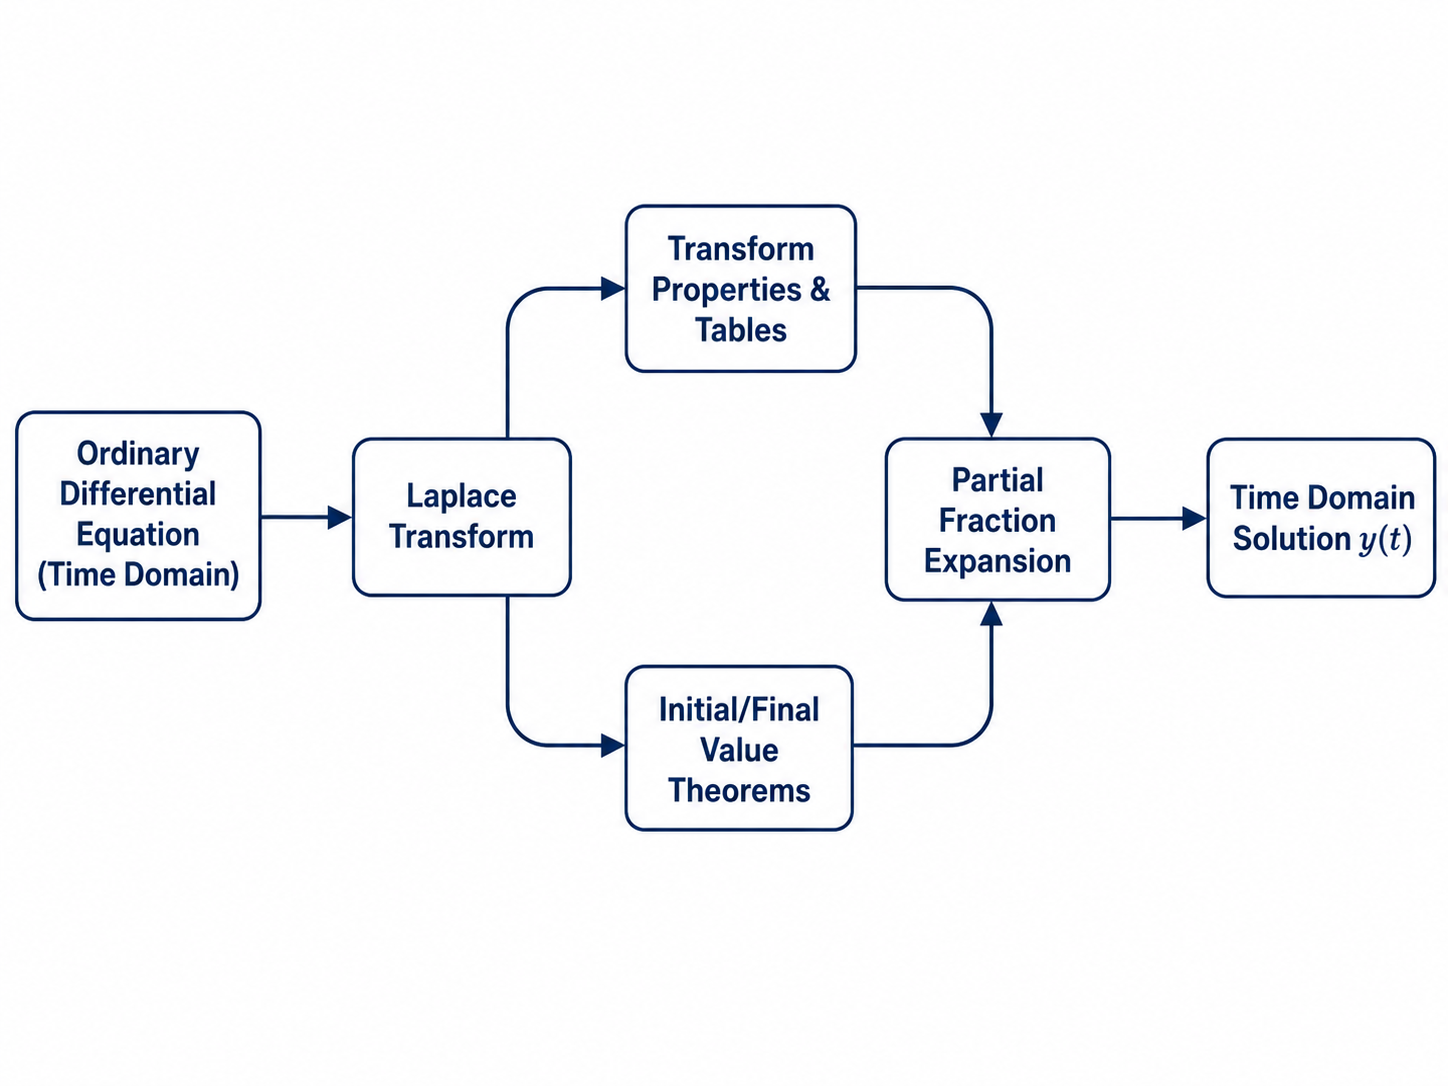
\includegraphics[width=0.70\textwidth]{images/ch2/figure-1.png}
\caption{แผนภาพภาพรวมเนื้อหาบทที่ 2 (Concept Map)}
\label{fig:ch2-1}
\end{figure}

\subsection{ผลการเรียนรู้ที่คาดหวัง (Learning
Outcomes)}\label{uxe1cuxe25uxe01uxe32uxe23uxe40uxe23uxe22uxe19uxe23uxe17uxe04uxe32uxe14uxe2buxe27uxe07-learning-outcomes}

เมื่อศึกษาจบบทนี้ นักศึกษาจะสามารถ:

\begin{longtable}[]{@{}
  >{\raggedright\arraybackslash}p{(\columnwidth - 2\tabcolsep) * \real{0.1875}}
  >{\raggedright\arraybackslash}p{(\columnwidth - 2\tabcolsep) * \real{0.8125}}@{}}
\toprule\noalign{}
\begin{minipage}[b]{\linewidth}\raggedright
รหัส
\end{minipage} & \begin{minipage}[b]{\linewidth}\raggedright
ผลการเรียนรู้ที่คาดหวัง
\end{minipage} \\
\midrule\noalign{}
\endhead
\bottomrule\noalign{}
\endlastfoot
\textbf{LO1} & แก้สมการเชิงอนุพันธ์อันดับ 1 และอันดับ 2
โดยใช้การแปลงลาปลาซได้อย่างถูกต้อง \\
\textbf{LO2} & ใช้ตารางคู่แปลง คุณสมบัติของการแปลงลาปลาซ
และการแยกเศษส่วนย่อยได้อย่างคล่องแคล่ว \\
\textbf{LO3} & ประยุกต์ใช้ทฤษฎีบทค่าเริ่มต้น (IVT) และทฤษฎีบทค่าสุดท้าย (FVT)
กับปัญหาระบบควบคุมได้ \\
\textbf{LO4} & แปลงแบบจำลองทางคณิตศาสตร์จากโดเมนเวลา (Time Domain) สู่โดเมน
s (s-Domain) เพื่อเตรียมความพร้อมสำหรับการศึกษาฟังก์ชันถ่ายโอนในบทที่ 3 \\
\textbf{LO5} & ใช้คำสั่ง MATLAB \texttt{laplace()}, \texttt{ilaplace()},
และ \texttt{partfrac()} เพื่อตรวจสอบความถูกต้องของคำตอบที่คำนวณด้วยมือได้ \\
\end{longtable}

\begin{center}\rule{0.5\linewidth}{0.5pt}\end{center}

\subsection{ทบทวนสมการเชิงอนุพันธ์สามัญ (Ordinary Differential
Equations)}\label{uxe17uxe1auxe17uxe27uxe19uxe2auxe21uxe01uxe32uxe23uxe40uxe0auxe07uxe2duxe19uxe1euxe19uxe18uxe2auxe32uxe21uxe0d-ordinary-differential-equations}

\textbf{สมการเชิงอนุพันธ์สามัญ (Ordinary Differential Equation, ODE)}
คือสมการทางคณิตศาสตร์ที่แสดงความสัมพันธ์ระหว่างฟังก์ชัน \(y(t)\)
กับอนุพันธ์ของฟังก์ชันนั้นเทียบกับเวลา \(t\) ในบริบทของวิศวกรรมระบบควบคุม ODE
ทำหน้าที่เป็น \textbf{``ภาษาทางคณิตศาสตร์''} ที่ใช้อธิบายพฤติกรรมของระบบกายภาพ
ตั้งแต่วงจรไฟฟ้าอย่างง่าย (RC) ไปจนถึงระบบไฟฟ้า-กลที่ซับซ้อน เช่น มอเตอร์ไฟฟ้ากระแสตรง
(DC Motor)

\begin{quote}
\textbf{หมายเหตุสำหรับผู้เรียนสายสามัญ (ม.6):} หากยังไม่เคยศึกษา ODE
อย่างเป็นระบบมาก่อน ขอแนะนำให้ทบทวนเนื้อหาในหัวข้อนี้อย่างละเอียด และฝึกทำแบบฝึกหัดข้อที่
1--2 ในหัวข้อ 2.9 ก่อนเข้าสู่เนื้อหาการแปลงลาปลาซ
\end{quote}

\subsubsection{สมการเชิงอนุพันธ์อันดับที่ 1 (First-Order
ODE)}\label{uxe2auxe21uxe01uxe32uxe23uxe40uxe0auxe07uxe2duxe19uxe1euxe19uxe18uxe2duxe19uxe14uxe1auxe17-1-first-order-ode}

รูปแบบทั่วไปของสมการเชิงอนุพันธ์อันดับ 1 ที่พบบ่อยในระบบควบคุม เขียนได้ดังนี้

\[\tau \frac{dy}{dt} + y(t) = K \cdot u(t)\]

โดยที่ตัวแปรในสมการมีความหมายดังนี้:

\begin{itemize}
\tightlist
\item
  \(\tau\) คือ \textbf{ค่าคงเวลา (Time Constant)} มีหน่วยเป็นวินาที
\item
  \(K\) คือ \textbf{อัตราขยาย (Gain)} ของระบบ
\item
  \(u(t)\) คือ สัญญาณอินพุตที่ป้อนเข้าสู่ระบบ
\end{itemize}

\textbf{ตัวอย่างระบบทางกายภาพที่อธิบายด้วย ODE อันดับ 1:}

\begin{itemize}
\tightlist
\item
  \textbf{วงจร RC:} \(RC\dfrac{dv_C}{dt} + v_C(t) = v_{in}(t)\) ซึ่งให้
  \(\tau = RC\)
\item
  \textbf{ระบบถ่ายเทความร้อน:} \(\tau\dfrac{dT}{dt} + T = T_{env}\) ซึ่งให้
  \(\tau = mC/hA\)
\item
  \textbf{มอเตอร์ DC (สมการวงจรกระแส):} \(L\dfrac{di}{dt} + Ri = v(t)\)
\end{itemize}

\textbf{คำตอบทั่วไปของ ODE อันดับ 1} (กรณีที่ \(u(t)\) เป็นค่าคงที่ และเงื่อนไขเริ่มต้น
\(y(0) = y_0\)):

\[\boxed{y(t) = (y_0 - y_\infty)\,e^{-t/\tau} + y_\infty}\]

โดยที่ \(y_\infty = K \cdot u\) คือค่าที่ระบบเข้าสู่ \textbf{สภาวะอยู่ตัว (Steady
State)}

\subsubsection{สมการเชิงอนุพันธ์อันดับที่ 2 (Second-Order
ODE)}\label{uxe2auxe21uxe01uxe32uxe23uxe40uxe0auxe07uxe2duxe19uxe1euxe19uxe18uxe2duxe19uxe14uxe1auxe17-2-second-order-ode}

รูปแบบมาตรฐาน (Standard Form) ของสมการเชิงอนุพันธ์อันดับ 2
ที่ใช้อธิบายระบบควบคุมส่วนใหญ่ เขียนได้ดังนี้

\[\boxed{\frac{d^2y}{dt^2} + 2\zeta\omega_n\frac{dy}{dt} + \omega_n^2\,y = K\omega_n^2\,u(t)}\]

โดยที่:

\begin{itemize}
\tightlist
\item
  \(\zeta\) (Zeta) คือ \textbf{อัตราส่วนหน่วง (Damping Ratio)} ซึ่งเป็นค่าที่ไม่มีมิติ
  (Dimensionless)
\item
  \(\omega_n\) คือ \textbf{ความถี่ธรรมชาติ (Natural Frequency)} มีหน่วยเป็น
  rad/s
\end{itemize}

\textbf{การจำแนกประเภทของระบบอันดับ 2 ตามค่า \(\zeta\):}

\begin{longtable}[]{@{}
  >{\raggedright\arraybackslash}p{(\columnwidth - 4\tabcolsep) * \real{0.1633}}
  >{\raggedright\arraybackslash}p{(\columnwidth - 4\tabcolsep) * \real{0.3878}}
  >{\raggedright\arraybackslash}p{(\columnwidth - 4\tabcolsep) * \real{0.4490}}@{}}
\toprule\noalign{}
\begin{minipage}[b]{\linewidth}\raggedright
ประเภท
\end{minipage} & \begin{minipage}[b]{\linewidth}\raggedright
เงื่อนไข \(\zeta\)
\end{minipage} & \begin{minipage}[b]{\linewidth}\raggedright
พฤติกรรมการตอบสนอง
\end{minipage} \\
\midrule\noalign{}
\endhead
\bottomrule\noalign{}
\endlastfoot
\textbf{Underdamped (หน่วงน้อย)} & \(0 < \zeta < 1\) & สั่นแบบหน่วงลดลง
(Damped Oscillation) --- พบในระบบส่วนใหญ่ \\
\textbf{Critically Damped (หน่วงวิกฤต)} & \(\zeta = 1\) & ไม่สั่น
และตอบสนองเร็วที่สุดโดยไม่เกินค่า (Overshoot) \\
\textbf{Overdamped (หน่วงมาก)} & \(\zeta > 1\) & ไม่สั่น
แต่ตอบสนองช้ากว่ากรณีหน่วงวิกฤต \\
\textbf{Undamped (ไม่มีการหน่วง)} & \(\zeta = 0\) & สั่นต่อเนื่องไม่หยุด
ซึ่งไม่เสถียรในทางปฏิบัติ \\
\end{longtable}

\begin{figure}[H]
\centering
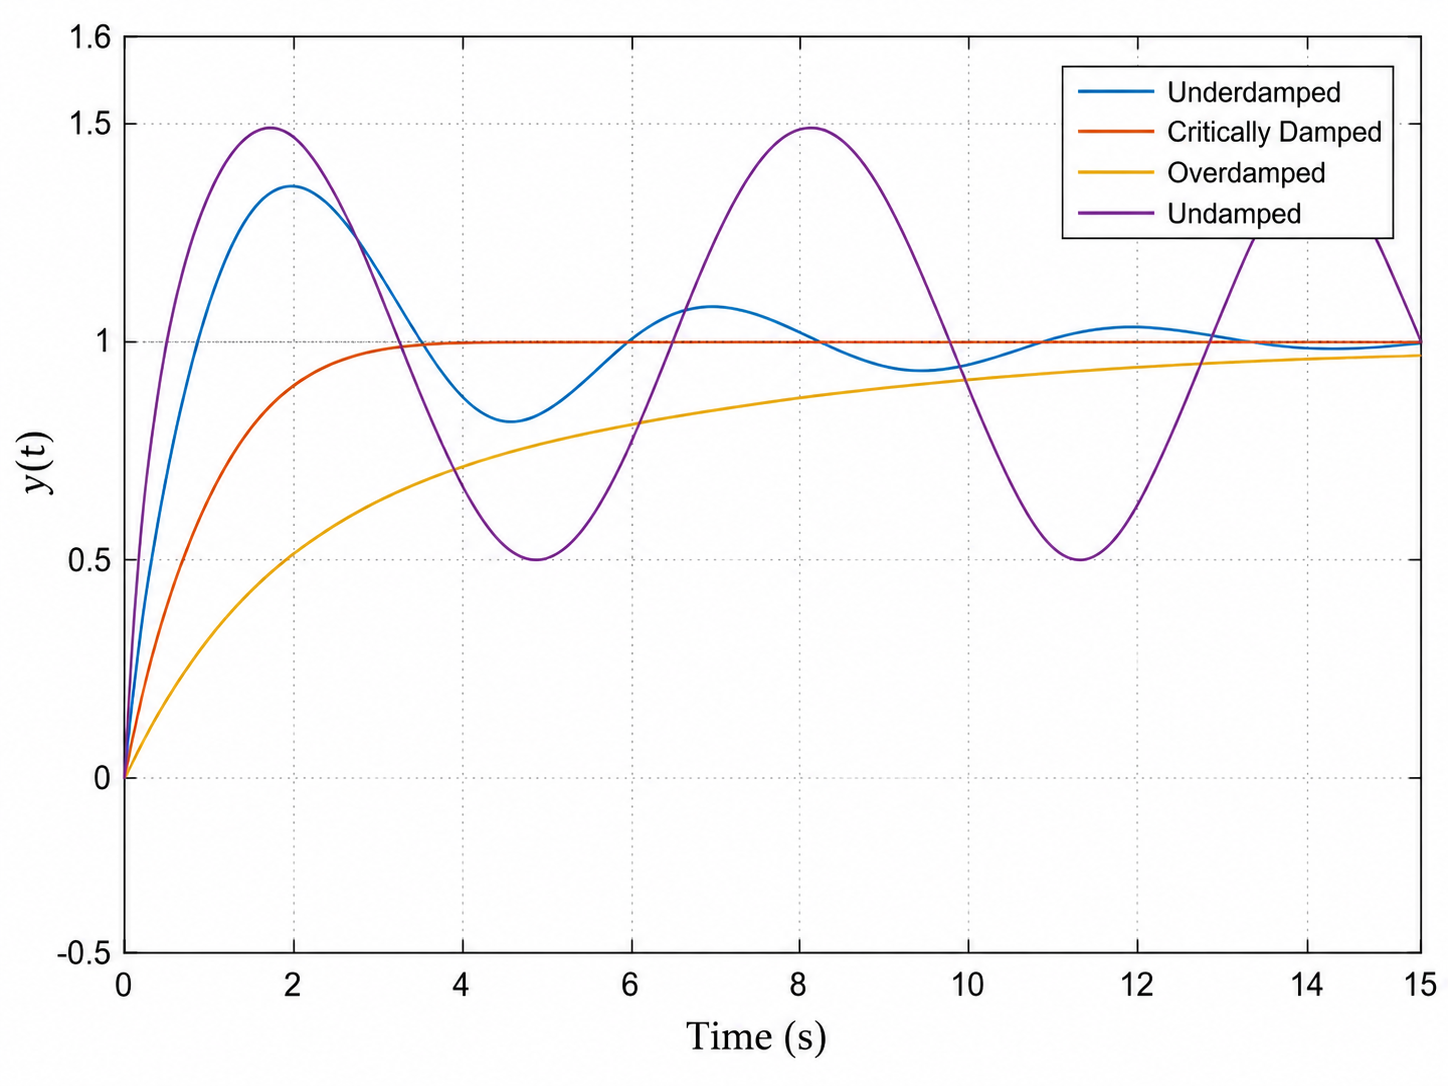
\includegraphics[width=0.70\textwidth]{images/ch2/figure-2.png}
\caption{กราฟเปรียบเทียบการตอบสนองของระบบอันดับ 2 ทั้ง 4 ประเภท}
\label{fig:ch2-2}
\end{figure}

\begin{quote}
\textbf{ตัวอย่างที่ 2.1 --- การเขียนสมการเชิงอนุพันธ์ของวงจร RLC อนุกรม}

\textbf{โจทย์:} วงจร RLC แบบอนุกรม (\(R=2\,\Omega\), \(L=1\,\text{H}\),
\(C=0.25\,\text{F}\)) ต่อกับแหล่งจ่ายแรงดัน \(v(t) = u(t)\) โวลต์
จงเขียนสมการเชิงอนุพันธ์ของกระแส \(i(t)\)

\textbf{วิธีทำ:}

\begin{enumerate}
\def\labelenumi{\arabic{enumi}.}
\tightlist
\item
  ใช้กฎ KVL:
  \(\displaystyle v(t) = L\frac{di}{dt} + Ri + \frac{1}{C}\int i\,dt\)
\item
  หาอนุพันธ์ทั้งสองข้าง:
  \(\displaystyle \frac{dv}{dt} = L\frac{d^2i}{dt^2} + R\frac{di}{dt} + \frac{i}{C}\)
\item
  แทนค่าพารามิเตอร์:
  \(\displaystyle \frac{d^2i}{dt^2} + 2\frac{di}{dt} + 4i = \frac{dv}{dt}\)
\item
  เมื่อ \(v(t) = u(t)\) จะได้ \(\dfrac{dv}{dt} = \delta(t)\) ดังนั้น
  \(\displaystyle \frac{d^2i}{dt^2} + 2\frac{di}{dt} + 4i = \delta(t)\)
\end{enumerate}

\textbf{การระบุพารามิเตอร์:}
\(2\zeta\omega_n = 2 \Rightarrow \zeta\omega_n = 1\) และ
\(\omega_n^2 = 4 \Rightarrow \omega_n = 2\) rad/s ดังนั้น \(\zeta = 0.5\)
ซึ่งจัดอยู่ในประเภท \textbf{Underdamped}
\end{quote}


\begin{figure}[H]
\centering
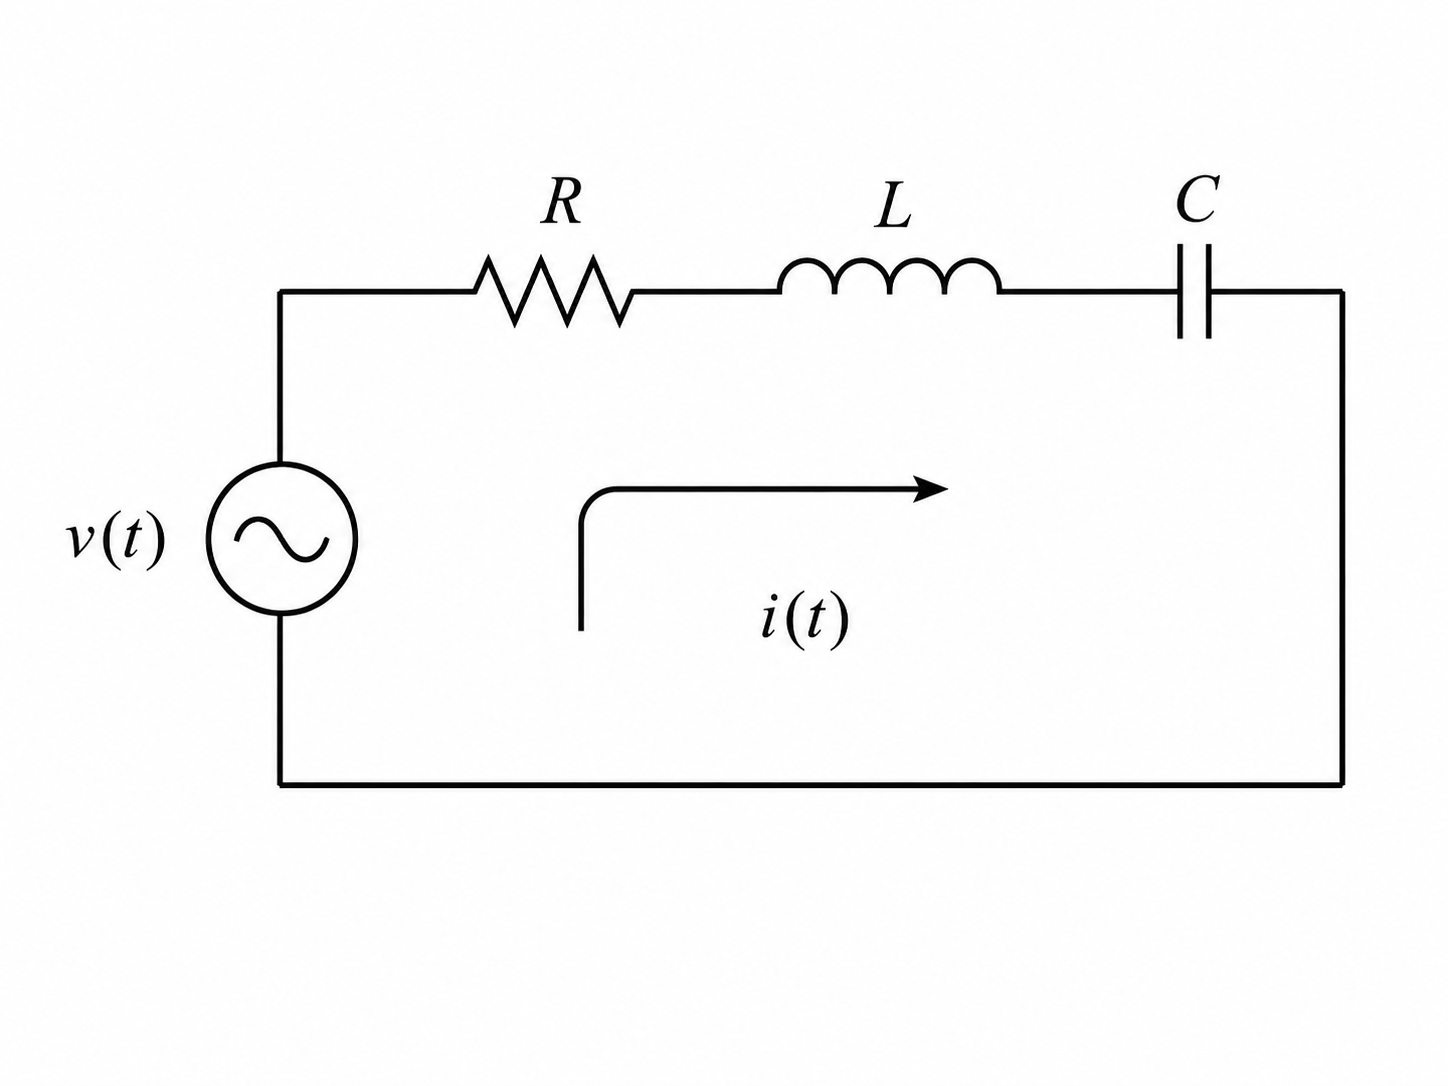
\includegraphics[width=0.50\textwidth]{images/ch2/figure-3.png}
\caption{แผนภาพวงจร RLC อนุกรม}
\label{fig:ch2-3}
\end{figure}

\begin{center}\rule{0.5\linewidth}{0.5pt}\end{center}

\subsection{การแปลงลาปลาซ (Laplace
Transform)}\label{uxe01uxe32uxe23uxe41uxe1buxe25uxe07uxe25uxe32uxe1buxe25uxe32uxe0b-laplace-transform}

\textbf{การแปลงลาปลาซ (Laplace Transform)}
เป็นเครื่องมือทางคณิตศาสตร์ที่ใช้แปลงสมการเชิงอนุพันธ์ (ODE) ในโดเมนเวลา (Time
Domain) ให้กลายเป็นสมการพีชคณิตในโดเมนเชิงซ้อน (s-Domain)
ซึ่งทำให้การแก้สมการมีความสะดวกและเป็นระบบมากยิ่งขึ้น

\subsubsection{นิยามของการแปลงลาปลาซ
(Definition)}\label{uxe19uxe22uxe32uxe21uxe02uxe2duxe07uxe01uxe32uxe23uxe41uxe1buxe25uxe07uxe25uxe32uxe1buxe25uxe32uxe0b-definition}

\[\boxed{F(s) = \mathcal{L}\{f(t)\} = \int_0^{\infty} f(t)\,e^{-st}\,dt}\]

โดยที่ \(s = \sigma + j\omega\) คือ \textbf{ตัวแปรเชิงซ้อน (Complex Variable)}
และ \(\sigma, \omega \in \mathbb{R}\)

\textbf{สัญลักษณ์ที่ใช้บ่อยในรายวิชานี้:}

\begin{itemize}
\tightlist
\item
  \(\mathcal{L}\{f(t)\} = F(s)\) --- การแปลงฟังก์ชันเวลา \(f(t)\) สู่ฟังก์ชัน
  \(F(s)\) ในโดเมน \(s\)
\item
  \(\mathcal{L}^{-1}\{F(s)\} = f(t)\) --- การแปลงกลับ (Inverse Laplace
  Transform)
\item
  \(f(t) \leftrightarrow F(s)\) --- สัญลักษณ์แสดงคู่แปลง
\end{itemize}

\begin{quote}
\textbf{เงื่อนไขการมีอยู่ (Existence Conditions):}
\begin{itemize}
\tightlist
\item \(f(t) = 0\) สำหรับ \(t < 0\) (สัญญาณเชิงเหตุ หรือ Causal Signal)
\item \(\displaystyle\int_0^\infty |f(t)|\,e^{-\sigma t}\,dt < \infty\)
สำหรับค่า \(\sigma\) บางค่า (เรียกว่า ROC หรือ Region of Convergence)
\end{itemize}

ในระบบควบคุม เงื่อนไขเหล่านี้มักเป็นจริงเสมอสำหรับสัญญาณที่นักศึกษาจะพบในรายวิชานี้
\end{quote}

\begin{figure}[H]
\centering
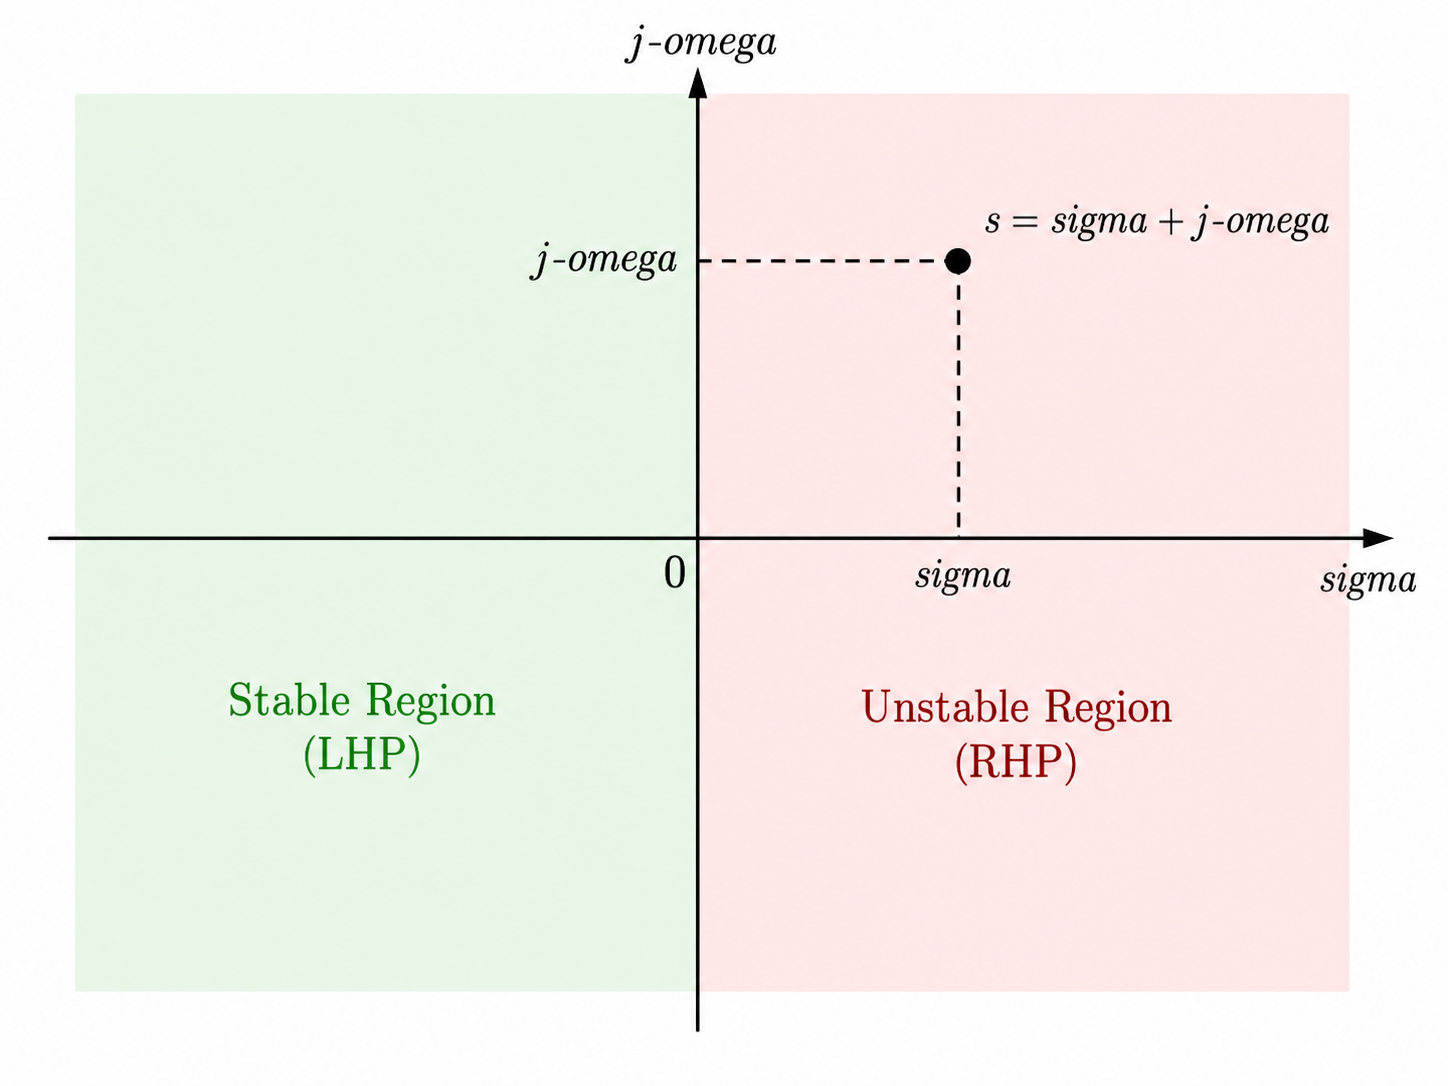
\includegraphics[width=0.70\textwidth]{images/ch2/figure-4.png}
\caption{ระนาบ s (s-Plane) และตัวแปรเชิงซ้อน}
\label{fig:ch2-4}
\end{figure}

\subsubsection{คุณสมบัติสำคัญของการแปลงลาปลาซ
(Properties)}\label{uxe04uxe13uxe2auxe21uxe1auxe15uxe2auxe33uxe04uxe0duxe02uxe2duxe07uxe01uxe32uxe23uxe41uxe1buxe25uxe07uxe25uxe32uxe1buxe25uxe32uxe0b-properties}

\begin{longtable}[]{@{}
  >{\raggedright\arraybackslash}p{(\columnwidth - 4\tabcolsep) * \real{0.2821}}
  >{\raggedright\arraybackslash}p{(\columnwidth - 4\tabcolsep) * \real{0.1538}}
  >{\raggedright\arraybackslash}p{(\columnwidth - 4\tabcolsep) * \real{0.5641}}@{}}
\toprule\noalign{}
\begin{minipage}[b]{\linewidth}\raggedright
คุณสมบัติ
\end{minipage} & \begin{minipage}[b]{\linewidth}\raggedright
สูตร
\end{minipage} & \begin{minipage}[b]{\linewidth}\raggedright
หมายเหตุ / ประโยชน์
\end{minipage} \\
\midrule\noalign{}
\endhead
\bottomrule\noalign{}
\endlastfoot
\textbf{เชิงเส้น (Linearity)} &
\(\mathcal{L}\{af(t)+bg(t)\} = aF(s)+bG(s)\) & สามารถแยกแปลงทีละเทอมได้ \\
\textbf{อนุพันธ์ครั้งที่ 1} & \(\mathcal{L}\{f'(t)\} = sF(s) - f(0^-)\) &
สำคัญมาก --- แปลง \(dy/dt\) ให้เป็น \(s\) \\
\textbf{อนุพันธ์ครั้งที่ 2} &
\parbox[t]{\linewidth}{\raggedright
\(\mathcal{L}\{f''(t)\} = s^2F(s)\)\\
\(\hspace*{1.5em} - sf(0^-) - f'(0^-)\)
} &
เงื่อนไขเริ่มต้นปรากฏเป็น \(f(0), f'(0)\) \\
\textbf{อินทิกรัล} &
\parbox[t]{\linewidth}{\raggedright
\(\mathcal{L}\{\int_0^t f(\tau)\,d\tau\}\)\\
\(\hspace*{1.5em} = \frac{F(s)}{s}\)
}
& หารด้วย \(s\) ในโดเมน s \\
\textbf{Frequency Shift} & \(\mathcal{L}\{e^{-at}f(t)\} = F(s+a)\) &
เลื่อนแกน \(s\) ด้วยค่า \(a\) \\
\textbf{Time Shift} & \(\mathcal{L}\{f(t-a)u(t-a)\} = e^{-as}F(s)\) &
ใช้กับสัญญาณที่ล่าช้า \(a\) วินาที \\
\textbf{Scaling} &
\(\mathcal{L}\{f(at)\} = \dfrac{1}{a}F\!\left(\dfrac{s}{a}\right)\) &
ใช้กับการย่อ/ขยายแกนเวลา \\
\end{longtable}

\begin{quote}
\textbf{คุณสมบัติ ``อนุพันธ์'' คือหัวใจสำคัญของบทนี้}

เมื่อกำหนดให้เงื่อนไขเริ่มต้นเป็นศูนย์ (\(y(0^-) = 0\)):

\[\mathcal{L}\left\{\frac{dy}{dt}\right\} = s\,Y(s) \qquad \mathcal{L}\left\{\frac{d^2y}{dt^2}\right\} = s^2 Y(s) \qquad \mathcal{L}\left\{\frac{d^n y}{dt^n}\right\} = s^n Y(s)\]

คุณสมบัตินี้คือกลไกหลักที่แปลง ODE ให้กลายเป็น \textbf{สมการพีชคณิต}
ซึ่งแก้ได้ง่ายกว่ามากเมื่อเทียบกับการแก้สมการเชิงอนุพันธ์โดยตรง
\end{quote}

\begin{quote}
\textbf{ตัวอย่างที่ 2.2 --- การหาการแปลงลาปลาซจากนิยามโดยตรง}

\textbf{โจทย์:} จงหา \(\mathcal{L}\{e^{-at}\}\) โดยใช้นิยามโดยตรง (กำหนด
\(a > 0\))

\textbf{วิธีทำ:}

\begin{enumerate}
\def\labelenumi{\arabic{enumi}.}
\tightlist
\item
  \(\mathcal{L}\{e^{-at}\} = \displaystyle\int_0^{\infty} e^{-at}\cdot e^{-st}\,dt = \int_0^{\infty} e^{-(s+a)t}\,dt\)
\item
  \(= \left[\dfrac{-1}{s+a}\cdot e^{-(s+a)t}\right]_0^{\infty} = 0 - \left(\dfrac{-1}{s+a}\right) = \dfrac{1}{s+a}\)
\end{enumerate}

\textbf{ผลลัพธ์:} \(\mathcal{L}\{e^{-at}\} = \dfrac{1}{s+a}\) สำหรับ
\(\text{Re}(s) > -a\)
\end{quote}

\subsubsection{ตารางคู่แปลงลาปลาซที่ใช้บ่อย (Common Laplace Transform
Pairs)}\label{uxe15uxe32uxe23uxe32uxe07uxe04uxe41uxe1buxe25uxe07uxe25uxe32uxe1buxe25uxe32uxe0buxe17uxe43uxe0auxe1auxe2duxe22-common-laplace-transform-pairs}

\begin{longtable}[]{@{}
  >{\raggedright\arraybackslash}p{(\columnwidth - 6\tabcolsep) * \real{0.0494}}
  >{\raggedright\arraybackslash}p{(\columnwidth - 6\tabcolsep) * \real{0.2716}}
  >{\raggedright\arraybackslash}p{(\columnwidth - 6\tabcolsep) * \real{0.3827}}
  >{\raggedright\arraybackslash}p{(\columnwidth - 6\tabcolsep) * \real{0.2963}}@{}}
\toprule\noalign{}
\begin{minipage}[b]{\linewidth}\raggedright
ที่
\end{minipage} & \begin{minipage}[b]{\linewidth}\raggedright
\(f(t),\; t \geq 0\)
\end{minipage} & \begin{minipage}[b]{\linewidth}\raggedright
\(F(s) = \mathcal{L}\{f(t)\}\)
\end{minipage} & \begin{minipage}[b]{\linewidth}\raggedright
การใช้งานในระบบควบคุม
\end{minipage} \\
\midrule\noalign{}
\endhead
\bottomrule\noalign{}
\endlastfoot
1 & \(\delta(t)\) --- Impulse & \(1\) & ทดสอบ Impulse Response \\
2 & \(u(t)\) --- Unit Step & \(\dfrac{1}{s}\) & อินพุต Step มาตรฐาน \\
3 & \(t\) --- Ramp & \(\dfrac{1}{s^2}\) & อินพุต Ramp \\
4 & \(t^n\) --- Power & \(\dfrac{n!}{s^{n+1}}\) & อินพุตพหุนาม \\
5 & \(e^{-at}\) & \(\dfrac{1}{s+a}\) & Exponential --- พบมากที่สุด \\
6 & \(t\,e^{-at}\) & \(\dfrac{1}{(s+a)^2}\) & Critically Damped
Response \\
7 & \(\sin(\omega t)\) & \(\dfrac{\omega}{s^2+\omega^2}\) &
องค์ประกอบการสั่น (Oscillation) \\
8 & \(\cos(\omega t)\) & \(\dfrac{s}{s^2+\omega^2}\) & จุดอ้างอิงเฟส (Phase
Reference) \\
9 & \(e^{-at}\sin(\omega t)\) & \(\dfrac{\omega}{(s+a)^2+\omega^2}\) &
Underdamped 2nd-Order \\
10 & \(e^{-at}\cos(\omega t)\) & \(\dfrac{s+a}{(s+a)^2+\omega^2}\) &
Underdamped 2nd-Order \\
11 & \(1 - e^{-at}\) & \(\dfrac{a}{s(s+a)}\) & Step Response ของระบบอันดับ
1 \\
12 & \(1 - (1+at)e^{-at}\) & \(\dfrac{a^2}{s(s+a)^2}\) & Step Response
Critically Damped \\
\end{longtable}

\begin{figure}[H]
\centering
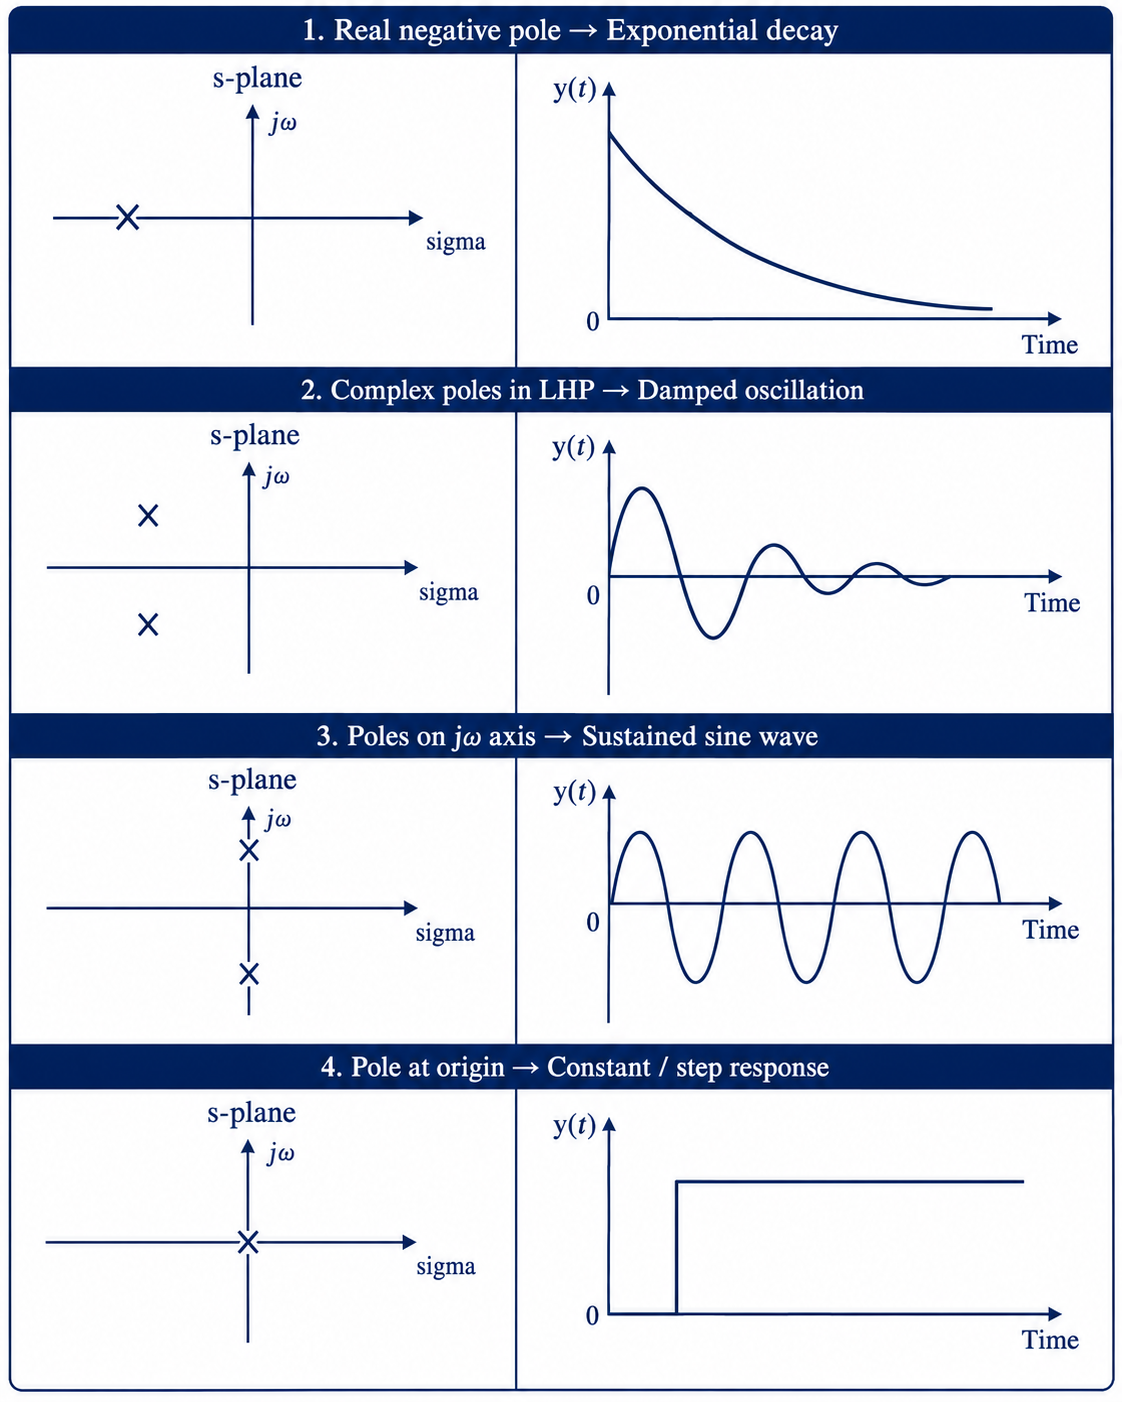
\includegraphics[width=0.70\textwidth]{images/ch2/figure-5.png}
\caption{ความสัมพันธ์ระหว่างตำแหน่งขั้ว (Pole) บนระนาบ s กับรูปร่างสัญญาณในโดเมนเวลา}
\label{fig:ch2-5}
\end{figure}

\subsection{ทฤษฎีบทค่าเริ่มต้นและค่าสุดท้าย (Value
Theorems)}\label{uxe17uxe24uxe29uxe0euxe1auxe17uxe04uxe32uxe40uxe23uxe21uxe15uxe19uxe41uxe25uxe30uxe04uxe32uxe2auxe14uxe17uxe32uxe22-value-theorems}

ทฤษฎีบททั้งสองข้อนี้ช่วยให้สามารถหาค่า \(f(t)\)
ที่ขอบของช่วงเวลาได้โดยไม่ต้องทำการแปลงกลับ (Inverse Laplace Transform) ก่อน
ซึ่งมีประโยชน์อย่างมากในการตรวจสอบความผิดพลาดสภาวะอยู่ตัว (Steady-State Error)
ของระบบควบคุม

\subsubsection{ทฤษฎีบทค่าเริ่มต้น (Initial Value Theorem,
IVT)}\label{uxe17uxe24uxe29uxe0euxe1auxe17uxe04uxe32uxe40uxe23uxe21uxe15uxe19-initial-value-theorem-ivt}

\[\boxed{\lim_{t \to 0^+} f(t) = \lim_{s \to \infty} \left[s\,F(s)\right]}\]

\textbf{เงื่อนไข:} ค่าลิมิต \(\lim_{s\to\infty}[sF(s)]\) ต้องสามารถหาค่าได้
(มีขีดจำกัด)

\textbf{ใช้เมื่อ:} ต้องการทราบค่าเริ่มต้นของการตอบสนอง \(y(0^+)\)
โดยไม่ต้องคำนวณการแปลงลาปลาซผกผัน

\subsubsection{ทฤษฎีบทค่าสุดท้าย (Final Value Theorem,
FVT)}\label{uxe17uxe24uxe29uxe0euxe1auxe17uxe04uxe32uxe2auxe14uxe17uxe32uxe22-final-value-theorem-fvt}

\[\boxed{\lim_{t \to \infty} f(t) = \lim_{s \to 0} \left[s\,F(s)\right]}\]

\begin{quote}
\textbf{ข้อควรระวัง:} \(sF(s)\) ต้องไม่มีขั้ว (Pole) อยู่บนแกน \(j\omega\)
หรือในระนาบขวา (Right-Half Plane) มิฉะนั้นผลลัพธ์ที่ได้จะไม่ถูกต้อง
\end{quote}

\textbf{ใช้เมื่อ:} ตรวจสอบค่าผลลัพธ์ในสภาวะอยู่ตัวของระบบควบคุม เช่น การหาค่า
\(y(\infty)\) ซึ่งคือค่าที่ระบบเข้าสู่สภาวะอยู่ตัวในที่สุด

\begin{figure}[H]
\centering
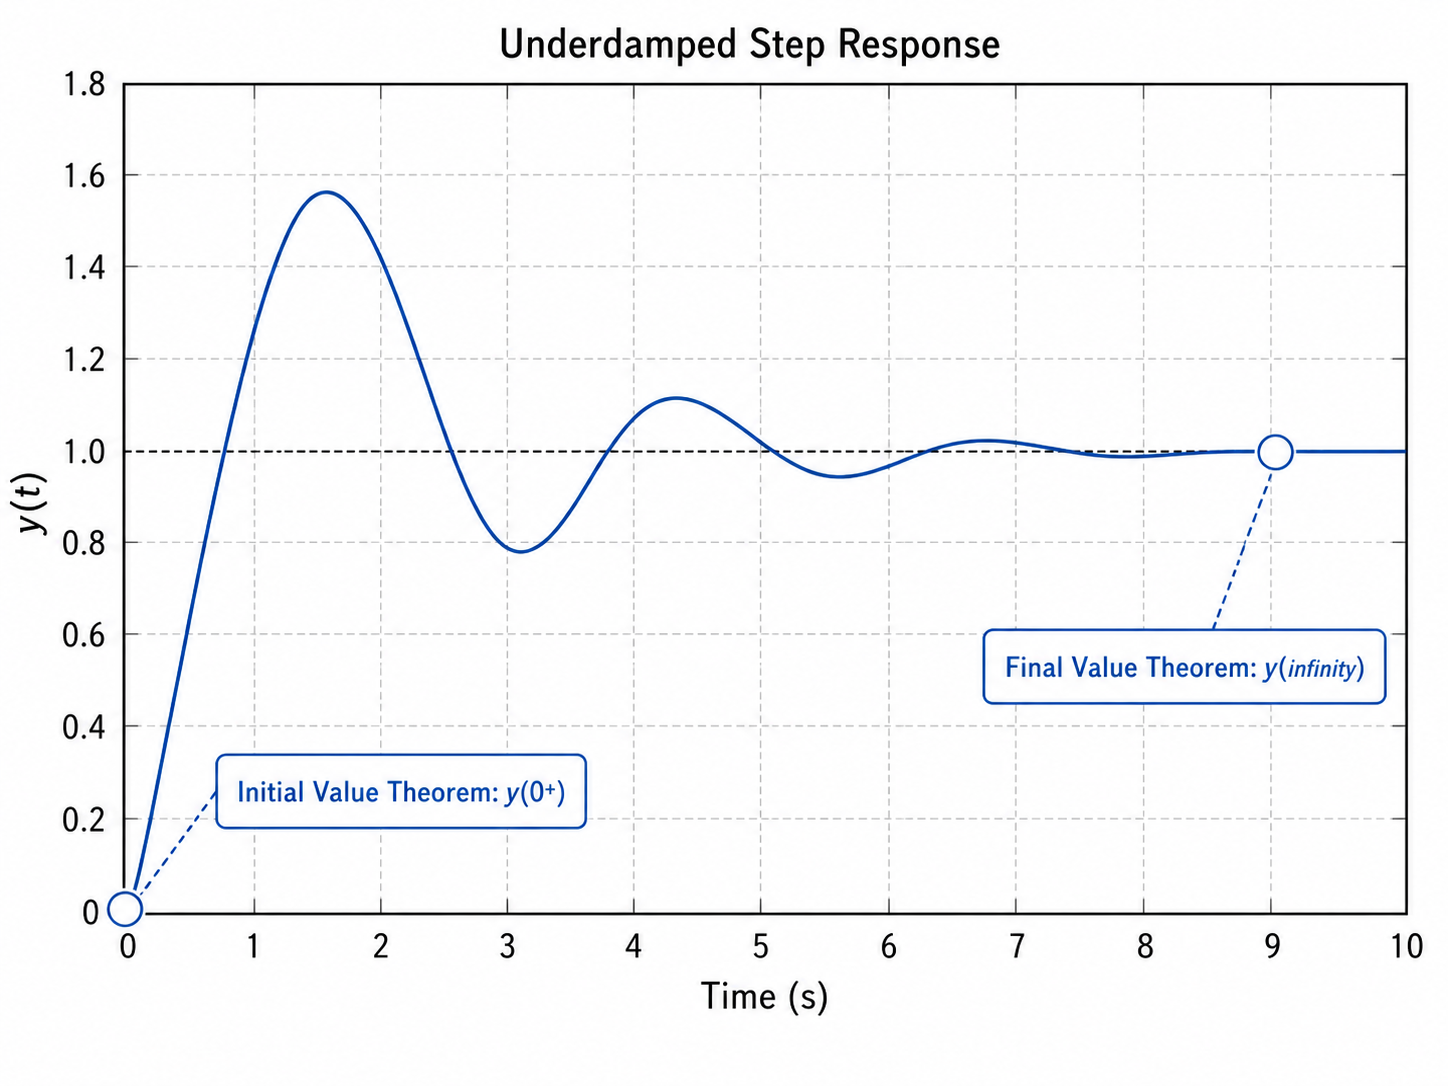
\includegraphics[width=0.70\textwidth]{images/ch2/figure-6.png}
\caption{แนวคิดเชิงกราฟของ IVT และ FVT}
\label{fig:ch2-6}
\end{figure}

\begin{quote}
\textbf{ตัวอย่างที่ 2.3 --- การประยุกต์ใช้ IVT และ FVT กับระบบควบคุม}

\textbf{โจทย์:} ระบบวงรอบปิด (Closed-loop) มีฟังก์ชันถ่ายโอน
\(\dfrac{Y(s)}{R(s)} = \dfrac{4}{(s+1)(s+4)}\) เมื่อรับอินพุตแบบ Unit Step
\(R(s) = 1/s\) จงหา (ก) ค่าเริ่มต้น \(y(0^+)\) และ (ข) ค่าสภาวะอยู่ตัว
\(y(\infty)\)

\textbf{วิธีทำ:}

หา \(Y(s)\):
\(\displaystyle Y(s) = \frac{1}{s} \cdot \frac{4}{(s+1)(s+4)} = \frac{4}{s(s+1)(s+4)}\)

\textbf{(ก) IVT:}
\(\displaystyle y(0^+) = \lim_{s\to\infty} s\,Y(s) = \lim_{s\to\infty} \frac{4}{(s+1)(s+4)} = 0\)
(สมเหตุสมผล เพราะระบบเริ่มจาก \(y=0\))

\textbf{(ข) FVT:}
\(\displaystyle y(\infty) = \lim_{s\to 0} s\,Y(s) = \lim_{s\to 0} \frac{4}{(s+1)(s+4)} = \frac{4}{1 \times 4} = 1\)
(ไม่มี Steady-State Error)

\textbf{ตรวจสอบเงื่อนไขการใช้ FVT:} Poles ของ \(sY(s)\) อยู่ที่ \(s = -1, -4\)
ซึ่งอยู่ในระนาบซ้าย (LHP) จึงสามารถใช้ FVT ได้
\end{quote}

\begin{center}\rule{0.5\linewidth}{0.5pt}\end{center}

\subsection{2.4 การแยกเศษส่วนย่อย (Partial Fraction Expansion ---
PFE)}\label{uxe01uxe32uxe23uxe41uxe22uxe01uxe40uxe28uxe29uxe2auxe27uxe19uxe22uxe2duxe22-partial-fraction-expansion-pfe}

การแยกเศษส่วนย่อยเป็นขั้นตอนสำคัญในการแปลงฟังก์ชัน \(F(s)\)
ให้อยู่ในรูปแบบที่สามารถใช้ตารางคู่แปลงหาการแปลงลาปลาซผกผันได้โดยตรง โดยทั่วไป
\(F(s) = N(s)/D(s)\) ซึ่งมีเงื่อนไขว่า \(\deg(N) < \deg(D)\)

\textbf{หลักการ:} แยกฟังก์ชัน \(F(s)\)
ที่มีรูปแบบซับซ้อนให้เป็นผลรวมของเศษส่วนย่อยที่มีรูปแบบทราบผลการแปลงลาปลาซผกผันอยู่แล้ว
แบ่งออกเป็น 3 กรณีหลัก ดังนี้

\begin{figure}[H]
\centering
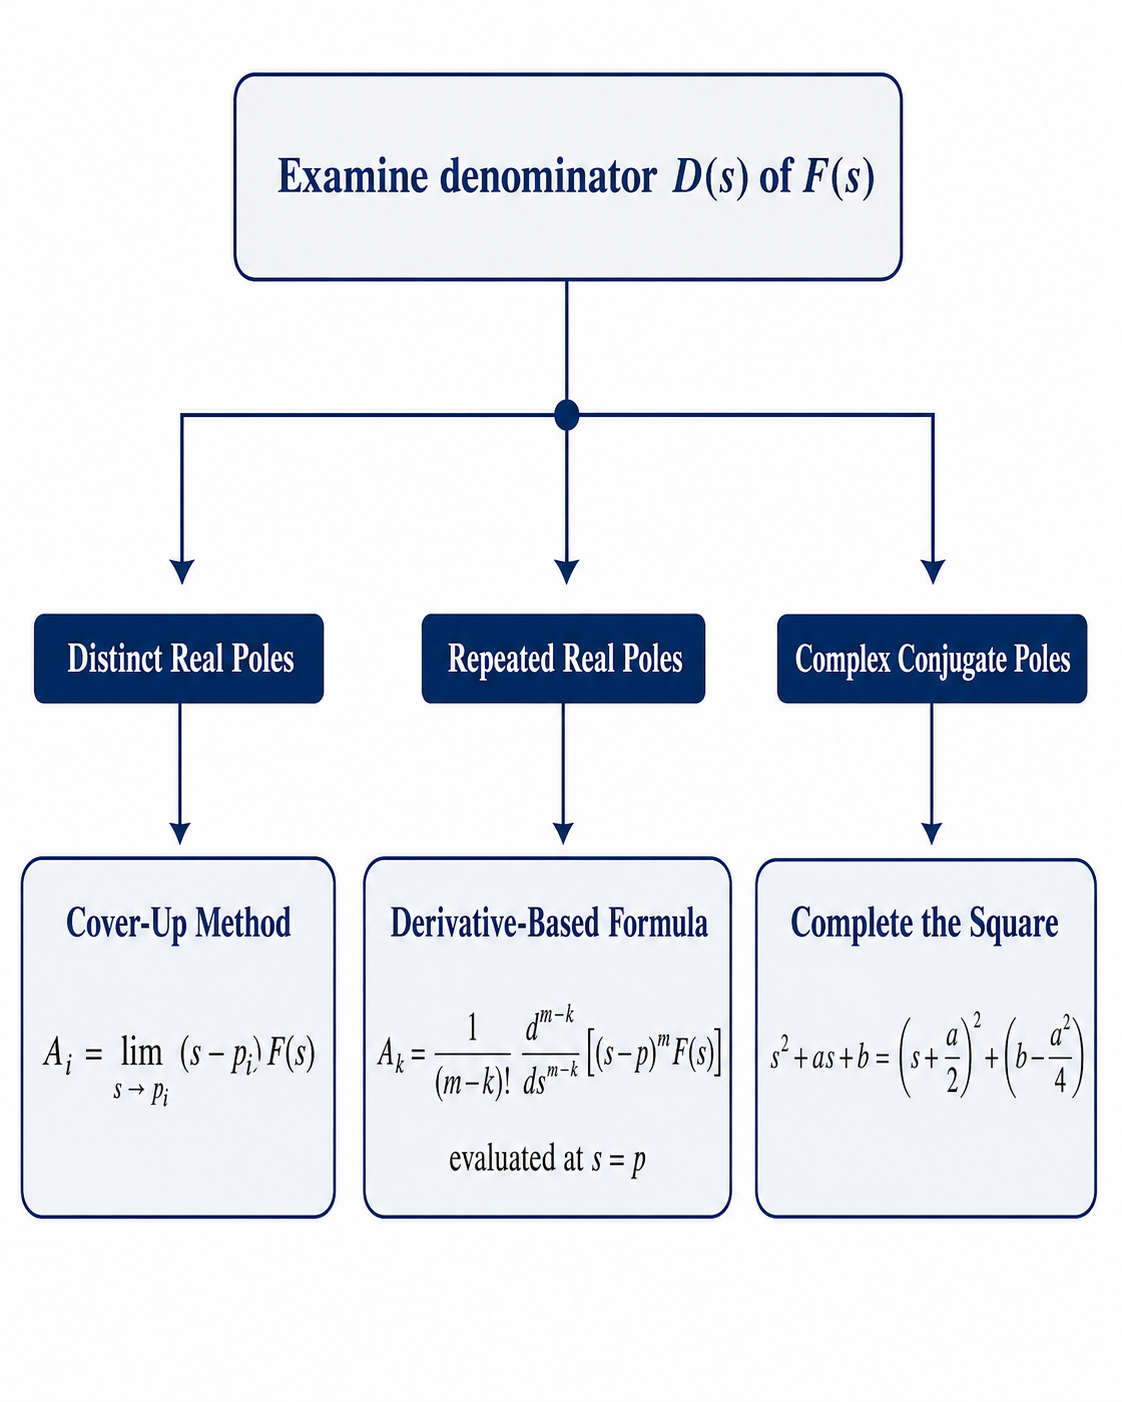
\includegraphics[width=0.70\textwidth]{images/ch2/figure-7.png}
\caption{แผนภาพการตัดสินใจเลือกวิธีแยกเศษส่วนย่อยตามประเภทของราก}
\label{fig:ch2-7}
\end{figure}

\subsubsection{กรณีที่ 1: รากจริงไม่ซ้ำ (Distinct Real
Poles)}\label{uxe01uxe23uxe13uxe17-1-uxe23uxe32uxe01uxe08uxe23uxe07uxe44uxe21uxe0buxe33-distinct-real-poles}

\[F(s) = \frac{N(s)}{(s+p_1)(s+p_2)\cdots(s+p_n)} = \frac{A_1}{s+p_1} + \frac{A_2}{s+p_2} + \cdots + \frac{A_n}{s+p_n}\]

หาสัมประสิทธิ์ \(A_i\) ด้วยวิธี \textbf{Cover-Up Method}:

\[A_i = \left[(s+p_i)\,F(s)\right]\Big|_{s = -p_i}\]

\begin{quote}
\textbf{ตัวอย่างที่ 2.4 --- PFE กรณีรากจริงไม่ซ้ำ}

\textbf{โจทย์:} จงหา
\(\mathcal{L}^{-1}\!\left\{\dfrac{s+3}{(s+1)(s+2)}\right\}\)

\textbf{วิธีทำ:} ตั้งรูปแบบ \(F(s) = \dfrac{A}{s+1} + \dfrac{B}{s+2}\)

หาค่า \(A = [(s+1)\,F(s)]\big|_{s=-1} = \dfrac{-1+3}{-1+2} = 2\)

หาค่า \(B = [(s+2)\,F(s)]\big|_{s=-2} = \dfrac{-2+3}{-2+1} = -1\)

ดังนั้น \(F(s) = \dfrac{2}{s+1} - \dfrac{1}{s+2}\) และแปลงกลับได้
\(\boxed{f(t) = 2e^{-t} - e^{-2t},\quad t \geq 0}\)

\textbf{ตรวจสอบด้วย MATLAB:}

\begin{Shaded}
\begin{Highlighting}[]
\VariableTok{syms} \VariableTok{s}\OperatorTok{;} \VariableTok{F} \OperatorTok{=}\NormalTok{ (}\VariableTok{s}\OperatorTok{+}\FloatTok{3}\NormalTok{)}\OperatorTok{/}\NormalTok{((}\VariableTok{s}\OperatorTok{+}\FloatTok{1}\NormalTok{)}\OperatorTok{*}\NormalTok{(}\VariableTok{s}\OperatorTok{+}\FloatTok{2}\NormalTok{))}\OperatorTok{;} \VariableTok{ilaplace}\NormalTok{(}\VariableTok{F}\NormalTok{)}
\end{Highlighting}
\end{Shaded}
\end{quote}

\subsubsection{กรณีที่ 2: รากซ้ำ (Repeated Real
Poles)}\label{uxe01uxe23uxe13uxe17-2-uxe23uxe32uxe01uxe0buxe33-repeated-real-poles}

\[F(s) = \frac{N(s)}{(s+p)^n} = \frac{A_1}{s+p} + \frac{A_2}{(s+p)^2} + \cdots + \frac{A_n}{(s+p)^n}\]

หาสัมประสิทธิ์ด้วยสูตร:

\[A_k = \frac{1}{(n-k)!}\left[\frac{d^{n-k}}{ds^{n-k}}(s+p)^n F(s)\right]\Bigg|_{s=-p}\]

\begin{quote}
\textbf{ตัวอย่างที่ 2.5 --- PFE กรณีรากซ้ำ}

\textbf{โจทย์:} จงหา
\(\mathcal{L}^{-1}\!\left\{\dfrac{2}{s(s+1)^2}\right\}\)

\textbf{วิธีทำ:} ตั้งรูปแบบ
\(F(s) = \dfrac{A}{s} + \dfrac{B}{s+1} + \dfrac{C}{(s+1)^2}\)

\(A = [s\,F(s)]\big|_{s=0} = 2\), ~
\(C = [(s+1)^2 F(s)]\big|_{s=-1} = -2\)

แทน \(s=1\) เพื่อหา \(B\):
\(\dfrac{2}{1\cdot 4} = \dfrac{2}{1} + \dfrac{B}{2} + \dfrac{-2}{4} \Rightarrow B = -2\)

ดังนั้น \(F(s) = \dfrac{2}{s} - \dfrac{2}{s+1} - \dfrac{2}{(s+1)^2}\)
และแปลงกลับได้ \(\boxed{f(t) = 2 - 2e^{-t} - 2te^{-t},\quad t \geq 0}\)
\end{quote}

\subsubsection{กรณีที่ 3: รากเชิงซ้อนคู่สังยุค (Complex Conjugate
Poles)}\label{uxe01uxe23uxe13uxe17-3-uxe23uxe32uxe01uxe40uxe0auxe07uxe0buxe2duxe19uxe04uxe2auxe07uxe22uxe04-complex-conjugate-poles}

\[F(s) = \frac{N(s)}{(s+a)^2 + \omega^2} = \frac{A(s+a) + B\omega}{(s+a)^2 + \omega^2}\]

\[\mathcal{L}^{-1}\{\cdots\} = A\,e^{-at}\cos(\omega t) + B\,e^{-at}\sin(\omega t)\]

(อ้างอิงคู่แปลงหมายเลข 9 และ 10 จากตารางในหัวข้อ 2.2.3)

\begin{quote}
\textbf{ตัวอย่างที่ 2.6 --- PFE กรณีรากเชิงซ้อน}

\textbf{โจทย์:} จงหา
\(\mathcal{L}^{-1}\!\left\{\dfrac{2s+3}{s^2+4s+5}\right\}\)

\textbf{วิธีทำ:}

\begin{enumerate}
\def\labelenumi{\arabic{enumi}.}
\tightlist
\item
  Complete the Square:
  \(s^2+4s+5 = (s+2)^2+1 \Rightarrow a=2,\;\omega=1\)
\item
  แยกตัวเศษ: \(2s+3 = 2(s+2) + (3-4) = 2(s+2) - 1\)
\item
  ดังนั้น
  \(\displaystyle F(s) = \frac{2(s+2)}{(s+2)^2+1} - \frac{1}{(s+2)^2+1}\)
\item
  แปลงกลับ:
  \(\boxed{f(t) = 2e^{-2t}\cos(t) - e^{-2t}\sin(t),\quad t \geq 0}\)
\end{enumerate}

\textbf{ตรวจสอบด้วย MATLAB:}

\begin{Shaded}
\begin{Highlighting}[]
\VariableTok{syms} \VariableTok{s}\OperatorTok{;} \VariableTok{F} \OperatorTok{=}\NormalTok{ (}\FloatTok{2}\OperatorTok{*}\VariableTok{s}\OperatorTok{+}\FloatTok{3}\NormalTok{)}\OperatorTok{/}\NormalTok{(}\VariableTok{s}\OperatorTok{\^{}}\FloatTok{2}\OperatorTok{+}\FloatTok{4}\OperatorTok{*}\VariableTok{s}\OperatorTok{+}\FloatTok{5}\NormalTok{)}\OperatorTok{;} \VariableTok{ilaplace}\NormalTok{(}\VariableTok{F}\NormalTok{)}
\end{Highlighting}
\end{Shaded}
\end{quote}

\begin{center}\rule{0.5\linewidth}{0.5pt}\end{center}

\subsection{การแก้สมการเชิงอนุพันธ์ด้วยการแปลงลาปลาซ}\label{uxe01uxe32uxe23uxe41uxe01uxe2auxe21uxe01uxe32uxe23uxe40uxe0auxe07uxe2duxe19uxe1euxe19uxe18uxe14uxe27uxe22uxe01uxe32uxe23uxe41uxe1buxe25uxe07uxe25uxe32uxe1buxe25uxe32uxe0b}

การแก้สมการเชิงอนุพันธ์ (ODE) ด้วยวิธีการแปลงลาปลาซมีขั้นตอนที่เป็นระบบ สามารถทำซ้ำได้
และไม่จำเป็นต้องหาคำตอบส่วน Homogeneous และ Particular Solution
แยกกันเหมือนวิธีคลาสสิก

\begin{quote}
\textbf{ขั้นตอนการแก้ ODE ด้วยการแปลงลาปลาซ (4 ขั้นตอน)}

\begin{enumerate}
\def\labelenumi{\arabic{enumi}.}
\tightlist
\item
  \textbf{แปลง ODE สู่ s-domain} โดยใช้คุณสมบัติอนุพันธ์ (รวมเงื่อนไขเริ่มต้น)
\item
  \textbf{แก้หา \(Y(s)\)} โดยการจัดรูปสมการพีชคณิต
\item
  \textbf{แยก \(Y(s)\)} ด้วยวิธีการแยกเศษส่วนย่อย (Partial Fraction
  Expansion)
\item
  \textbf{แปลงกลับ} จาก \(Y(s)\) สู่ \(y(t)\) โดยใช้ตารางคู่แปลง
\end{enumerate}
\end{quote}

\begin{quote}
\textbf{ตัวอย่างที่ 2.7 --- แก้ ODE อันดับ 1 ด้วยการแปลงลาปลาซ}

\textbf{โจทย์:} แก้สมการ \(\dfrac{dy}{dt} + 2y = 3u(t)\) โดย \(y(0) = 1\)
และ \(u(t)\) คือ Unit Step

\textbf{ขั้น 1:} \([sY(s) - 1] + 2Y(s) = \dfrac{3}{s}\)

\textbf{ขั้น 2:}
\(Y(s)(s+2) = \dfrac{3}{s} + 1 \Rightarrow Y(s) = \dfrac{3}{s(s+2)} + \dfrac{1}{s+2}\)

\textbf{ขั้น 3:}
\(\dfrac{3}{s(s+2)} = \dfrac{3/2}{s} + \dfrac{-3/2}{s+2} \Rightarrow Y(s) = \dfrac{3/2}{s} - \dfrac{1/2}{s+2}\)

\textbf{ขั้น 4:}
\(\boxed{y(t) = \dfrac{3}{2} - \dfrac{1}{2}e^{-2t},\quad t \geq 0}\)

\textbf{ตรวจสอบ:} FVT ให้ \(\lim_{s\to 0}[s\,Y(s)] = 3/2\) \checkmark{} และ
\(y(0) = 3/2 - 1/2 = 1\) \checkmark{}
\end{quote}

\begin{quote}
\textbf{ตัวอย่างที่ 2.8 --- แก้ ODE อันดับ 2 ด้วยการแปลงลาปลาซ}

\textbf{โจทย์:} แก้สมการ
\(\dfrac{d^2y}{dt^2} + 3\dfrac{dy}{dt} + 2y = 2u(t)\) โดย
\(y(0) = 0,\; y'(0) = 0\)

\textbf{ขั้น 1:} \(s^2 Y(s) + 3s\,Y(s) + 2Y(s) = \dfrac{2}{s}\)

\textbf{ขั้น 2:}
\(Y(s)(s^2+3s+2) = \dfrac{2}{s} \Rightarrow Y(s) = \dfrac{2}{s(s+1)(s+2)}\)

\textbf{ขั้น 3:}
\(A = \dfrac{2}{(1)(2)} = 1,\; B = \dfrac{2}{(-1)(1)} = -2,\; C = \dfrac{2}{(-2)(-1)} = 1\)
\[Y(s) = \frac{1}{s} - \frac{2}{s+1} + \frac{1}{s+2}\]

\textbf{ขั้น 4:} \(\boxed{y(t) = 1 - 2e^{-t} + e^{-2t},\quad t \geq 0}\)

\textbf{ตรวจสอบ:} \(y(0) = 0\) \checkmark, \(y(\infty) = 1\) \checkmark,
\(y'(0) = 2-2 = 0\) \checkmark
\end{quote}

\begin{center}\rule{0.5\linewidth}{0.5pt}\end{center}

\subsection{ความสัมพันธ์ระหว่าง Time Domain และ
s-Domain}\label{uxe04uxe27uxe32uxe21uxe2auxe21uxe1euxe19uxe18uxe23uxe30uxe2buxe27uxe32uxe07-time-domain-uxe41uxe25uxe30-s-domain}

การเข้าใจความสัมพันธ์ระหว่างทั้งสองโดเมนนี้เป็นพื้นฐานสำคัญของวิศวกรรมระบบควบคุม
เพราะการวิเคราะห์และการออกแบบในบทถัดไปทั้งหมดจะดำเนินการในโดเมน s

\begin{longtable}[]{@{}
  >{\raggedright\arraybackslash}p{(\columnwidth - 4\tabcolsep) * \real{0.1905}}
  >{\raggedright\arraybackslash}p{(\columnwidth - 4\tabcolsep) * \real{0.3095}}
  >{\raggedright\arraybackslash}p{(\columnwidth - 4\tabcolsep) * \real{0.5000}}@{}}
\toprule\noalign{}
\begin{minipage}[b]{\linewidth}\raggedright
มุมมอง
\end{minipage} & \begin{minipage}[b]{\linewidth}\raggedright
Time Domain
\end{minipage} & \begin{minipage}[b]{\linewidth}\raggedright
s-Domain (Laplace)
\end{minipage} \\
\midrule\noalign{}
\endhead
\bottomrule\noalign{}
\endlastfoot
\textbf{ตัวแปร} & \(t\) (วินาที) & \(s = \sigma + j\omega\) (เชิงซ้อน) \\
\textbf{สมการของระบบ} & ODE (การแก้อนุพันธ์อาจยาก) & สมการพีชคณิต (แก้ได้ง่าย) \\
\textbf{การหาอนุพันธ์} & \(d/dt\) & คูณด้วย \(s\) \\
\textbf{การอินทิเกรต} & \(\int dt\) & หารด้วย \(s\) \\
\textbf{เงื่อนไขเริ่มต้น} & ต้องจัดการแยกในขั้นแก้สมการ & ปรากฏอัตโนมัติใน
\(Y(s)\) \\
\textbf{ฟังก์ชันถ่ายโอน} & ไม่ชัดเจน / ซับซ้อน & \(G(s) = Y(s)/U(s)\)
(ชัดเจนมาก) \\
\textbf{การวิเคราะห์เสถียรภาพ} & พิจารณาพฤติกรรม \(y(t)\) เมื่อ \(t\to\infty\)
& พิจารณาตำแหน่งของขั้ว (Poles) ใน s-plane \\
\textbf{การวิเคราะห์ความถี่} & ทำได้ยาก (ต้องใช้ Fourier Transform) & แทน
\(s = j\omega\) เพื่อสร้าง Bode Plot \\
\end{longtable}

\begin{quote}
\textbf{แนวคิดเชิงกายภาพ --- เพราะเหตุใดจึงต้องใช้ s-Domain}

พิจารณาระบบควบคุมมอเตอร์ไฟฟ้ากระแสตรงที่มีสมการเชิงอนุพันธ์คู่กัน:

\[J\frac{d\omega}{dt} + B\omega = K_t\,i(t) \qquad \text{และ} \qquad L\frac{di}{dt} + Ri = v(t) - K_b\,\omega\]

การแก้สมการเชิงอนุพันธ์คู่ที่มีตัวแปรไม่ทราบค่าสองตัว (\(\omega\) และ \(i\))
พร้อมกันในโดเมนเวลาทำได้ยากมาก แต่เมื่อแปลงสู่โดเมน s แล้ว สมการทั้งสองจะกลายเป็น

\begin{itemize}
\tightlist
\item
  \((Js + B)\Omega(s) = K_t\,I(s)\)
\item
  \((Ls + R)I(s) = V(s) - K_b\,\Omega(s)\)
\end{itemize}

ซึ่งเป็นระบบสมการพีชคณิตที่สามารถแก้ได้ทันที
นี่คือเหตุผลสำคัญที่วิศวกรระบบควบคุมทุกคนทำงานในโดเมน s เป็นหลัก
\end{quote}

\begin{figure}[H]
\centering
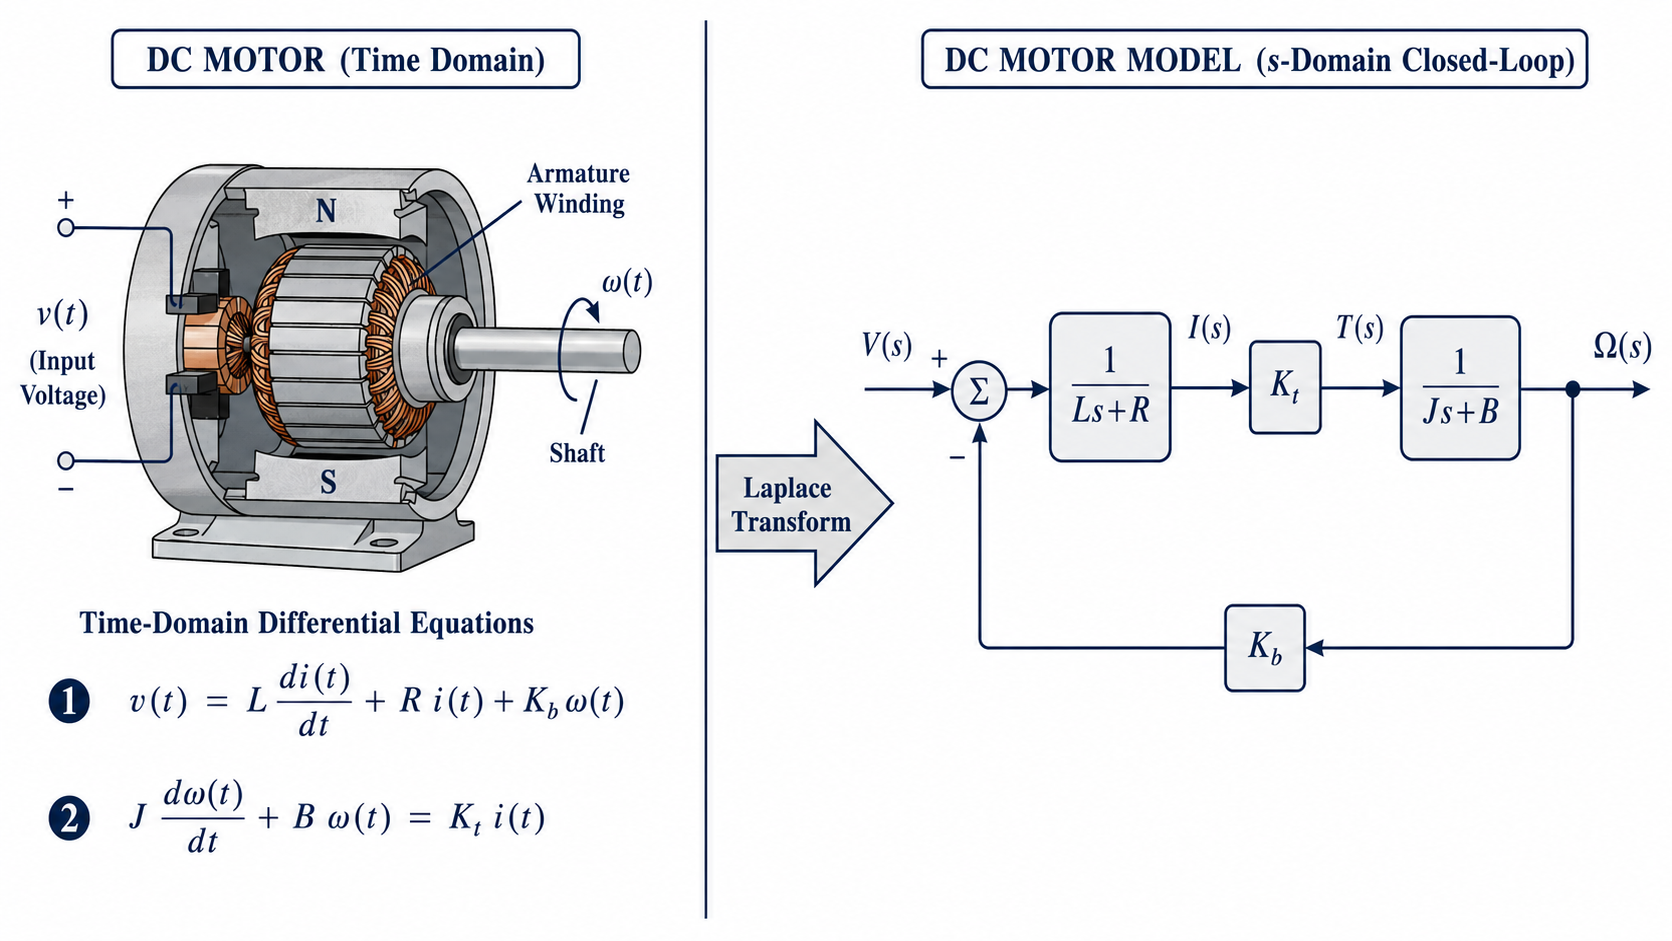
\includegraphics[width=0.70\textwidth]{images/ch2/figure-8.png}
\caption{ภาพประกอบที่ 8: บล็อกไดอะแกรมมอเตอร์ DC แสดงการแปลงจากโดเมนเวลาสู่โดเมน s}
\label{fig:ch2-8}
\end{figure}

\begin{quote}
\emph{คำอธิบายภาพ:} ภาพแบ่งเป็น 2 ส่วนซ้าย-ขวา
ส่วนซ้ายแสดงภาพตัดขวางเชิงแนวคิดของมอเตอร์ไฟฟ้ากระแสตรง
พร้อมป้ายกำกับสมการเชิงอนุพันธ์คู่ทั้งสองสมการ (สมการทางกล
\(J\dot\omega + B\omega = K_t i\) และสมการทางไฟฟ้า
\(L\dot i + Ri = v - K_b\omega\)) วางอยู่ใกล้ส่วนของมอเตอร์ที่เกี่ยวข้อง
(สมการทางไฟฟ้าใกล้ขดลวด สมการทางกลใกล้แกนหมุน) ส่วนขวาแสดงบล็อกไดอะแกรมในโดเมน
s ที่มีบล็อกสองบล็อกเชื่อมต่อกันแบบป้อนกลับ (Feedback Loop) แสดง
\(V(s) \to (Ls+R)^{-1} \to I(s) \to K_t \to (Js+B)^{-1} \to \Omega(s)\)
พร้อมเส้นป้อนกลับ \(K_b\)
มีลูกศรขนาดใหญ่เชื่อมจากภาพมอเตอร์ทางซ้ายไปยังบล็อกไดอะแกรมทางขวา พร้อมข้อความ
``Laplace Transform'' กำกับไว้บนลูกศร
เพื่อสื่อถึงการแปลงจากระบบจริงสู่แบบจำลองทางคณิตศาสตร์
\end{quote}

\subsection{กิจกรรมปฏิบัติการ (Laboratory
Activities)}\label{uxe01uxe08uxe01uxe23uxe23uxe21uxe1buxe0fuxe1auxe15uxe01uxe32uxe23-laboratory-activities}

ปฏิบัติการในหัวข้อนี้ใช้ MATLAB Symbolic Math Toolbox และ Simulink
เพื่อยืนยันความถูกต้องของผลการคำนวณที่ได้จากการคำนวณด้วยมือ

\subsubsection{ปฏิบัติการที่ 2-1: คำสั่งการแปลงลาปลาซใน
MATLAB}\label{uxe1buxe0fuxe1auxe15uxe01uxe32uxe23uxe17-2-1-uxe04uxe33uxe2auxe07uxe01uxe32uxe23uxe41uxe1buxe25uxe07uxe25uxe32uxe1buxe25uxe32uxe0buxe43uxe19-matlab}

\textbf{ขั้นตอนที่ 1 --- กำหนดตัวแปรสัญลักษณ์:}

\begin{Shaded}
\begin{Highlighting}[]
\VariableTok{syms} \VariableTok{s} \VariableTok{t} \VariableTok{a} \VariableTok{w}\OperatorTok{;}
\end{Highlighting}
\end{Shaded}

\textbf{ขั้นตอนที่ 2 --- หาการแปลงลาปลาซ:}

\begin{Shaded}
\begin{Highlighting}[]
\VariableTok{f} \OperatorTok{=} \FloatTok{3}\OperatorTok{*}\VariableTok{exp}\NormalTok{(}\OperatorTok{{-}}\FloatTok{2}\OperatorTok{*}\VariableTok{t}\NormalTok{) }\OperatorTok{+} \FloatTok{5}\OperatorTok{*}\VariableTok{sin}\NormalTok{(}\FloatTok{4}\OperatorTok{*}\VariableTok{t}\NormalTok{)}\OperatorTok{;}
\VariableTok{F} \OperatorTok{=} \VariableTok{laplace}\NormalTok{(}\VariableTok{f}\OperatorTok{,} \VariableTok{t}\OperatorTok{,} \VariableTok{s}\NormalTok{)   }\CommentTok{\% ผลลัพธ์: 3/(s+2) + 20/(s\^{}2+16)}
\end{Highlighting}
\end{Shaded}

\textbf{ขั้นตอนที่ 3 --- หาการแปลงลาปลาซผกผัน:}

\begin{Shaded}
\begin{Highlighting}[]
\VariableTok{F} \OperatorTok{=}\NormalTok{ (}\VariableTok{s}\OperatorTok{+}\FloatTok{3}\NormalTok{)}\OperatorTok{/}\NormalTok{((}\VariableTok{s}\OperatorTok{+}\FloatTok{1}\NormalTok{)}\OperatorTok{*}\NormalTok{(}\VariableTok{s}\OperatorTok{+}\FloatTok{2}\NormalTok{))}\OperatorTok{;}
\VariableTok{f} \OperatorTok{=} \VariableTok{ilaplace}\NormalTok{(}\VariableTok{F}\OperatorTok{,} \VariableTok{s}\OperatorTok{,} \VariableTok{t}\NormalTok{)  }\CommentTok{\% ผลลัพธ์: 2*exp({-}t) {-} exp({-}2t)}
\end{Highlighting}
\end{Shaded}

\textbf{ขั้นตอนที่ 4 --- การแยกเศษส่วนย่อย:}

\begin{Shaded}
\begin{Highlighting}[]
\VariableTok{F} \OperatorTok{=}\NormalTok{ (}\VariableTok{s}\OperatorTok{+}\FloatTok{3}\NormalTok{)}\OperatorTok{/}\NormalTok{((}\VariableTok{s}\OperatorTok{+}\FloatTok{1}\NormalTok{)}\OperatorTok{*}\NormalTok{(}\VariableTok{s}\OperatorTok{+}\FloatTok{2}\NormalTok{))}\OperatorTok{;}
\VariableTok{partfrac}\NormalTok{(}\VariableTok{F}\OperatorTok{,} \VariableTok{s}\NormalTok{)  }\CommentTok{\% แสดงเศษส่วนย่อย: 2/(s+1) {-} 1/(s+2)}
\end{Highlighting}
\end{Shaded}

\textbf{ขั้นตอนที่ 5 --- แก้ ODE และพล็อตกราฟ:}

\begin{Shaded}
\begin{Highlighting}[]
\VariableTok{Y} \OperatorTok{=}\NormalTok{ (}\FloatTok{3}\OperatorTok{/}\VariableTok{s} \OperatorTok{+} \FloatTok{1}\NormalTok{)}\OperatorTok{/}\NormalTok{(}\VariableTok{s}\OperatorTok{+}\FloatTok{2}\NormalTok{)}\OperatorTok{;}
\VariableTok{y} \OperatorTok{=} \VariableTok{ilaplace}\NormalTok{(}\VariableTok{Y}\OperatorTok{,} \VariableTok{s}\OperatorTok{,} \VariableTok{t}\NormalTok{)}\OperatorTok{;}
\VariableTok{t\_vec} \OperatorTok{=} \FloatTok{0}\OperatorTok{:}\FloatTok{0.01}\OperatorTok{:}\FloatTok{5}\OperatorTok{;}
\VariableTok{y\_vec} \OperatorTok{=} \VariableTok{double}\NormalTok{(}\VariableTok{subs}\NormalTok{(}\VariableTok{y}\OperatorTok{,} \VariableTok{t}\OperatorTok{,} \VariableTok{t\_vec}\NormalTok{))}\OperatorTok{;}
\VariableTok{plot}\NormalTok{(}\VariableTok{t\_vec}\OperatorTok{,} \VariableTok{y\_vec}\OperatorTok{,} \SpecialStringTok{\textquotesingle{}b{-}\textquotesingle{}}\OperatorTok{,} \SpecialStringTok{\textquotesingle{}LineWidth\textquotesingle{}}\OperatorTok{,} \FloatTok{2}\NormalTok{)}
\VariableTok{xlabel}\NormalTok{(}\SpecialStringTok{\textquotesingle{}เวลา t (วินาที)\textquotesingle{}}\NormalTok{)}\OperatorTok{;} \VariableTok{ylabel}\NormalTok{(}\SpecialStringTok{\textquotesingle{}y(t)\textquotesingle{}}\NormalTok{)}\OperatorTok{;} \VariableTok{grid} \VariableTok{on}
\VariableTok{title}\NormalTok{(}\SpecialStringTok{\textquotesingle{}Step Response: dy/dt + 2y = 3, y(0)=1\textquotesingle{}}\NormalTok{)}\OperatorTok{;}
\VariableTok{yline}\NormalTok{(}\FloatTok{1.5}\OperatorTok{,} \SpecialStringTok{\textquotesingle{}r{-}{-}\textquotesingle{}}\OperatorTok{,} \SpecialStringTok{\textquotesingle{}Steady State\textquotesingle{}}\NormalTok{)}
\end{Highlighting}
\end{Shaded}

\subsubsection{ปฏิบัติการที่ 2-2: การจำลองระบบใน
Simulink}\label{uxe1buxe0fuxe1auxe15uxe01uxe32uxe23uxe17-2-2-uxe01uxe32uxe23uxe08uxe33uxe25uxe2duxe07uxe23uxe30uxe1auxe1auxe43uxe19-simulink}

\textbf{ขั้นตอนการสร้างแบบจำลอง:}

\begin{enumerate}
\def\labelenumi{\arabic{enumi}.}
\tightlist
\item
  เปิด Simulink และสร้าง New Model
\item
  ลากบล็อก \texttt{Step\ (Sources)} \(\rightarrow\)
  \texttt{Transfer\ Fcn\ (Continuous)} \(\rightarrow\) \texttt{Scope}
\item
  สำหรับสมการ \(dy/dt + 2y = 3u(t)\): ตั้งค่า Transfer Function เป็น
  \texttt{3/(s+2)}
\item
  ตั้งค่า Step: Step Time = 0, Initial Value = 0, Final Value = 1
\item
  เชื่อมต่อบล็อก: Step \(\rightarrow\) Transfer Fcn \(\rightarrow\) Scope
\item
  รัน Simulation แล้วเปิด Scope เพื่อสังเกตกราฟ \(y(t)\)
\item
  เปรียบเทียบค่า \(y(\infty) = 3/2 = 1.5\) กับค่าที่ปรากฏบน Scope
\end{enumerate}

\begin{figure}[H]
\centering
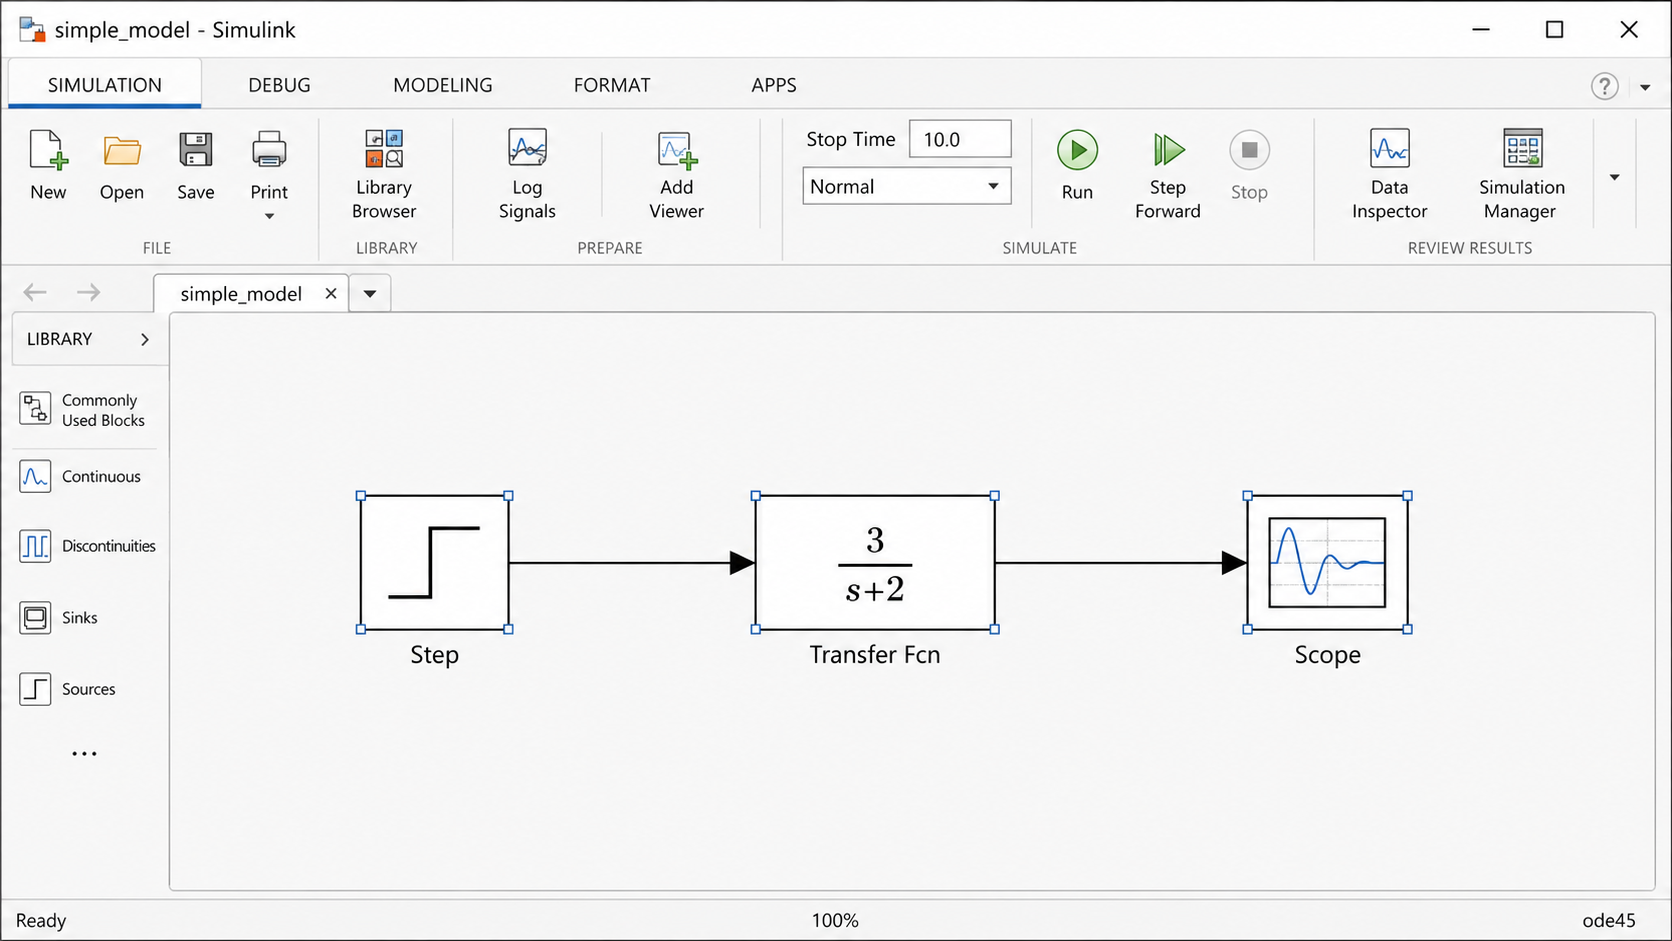
\includegraphics[width=0.70\textwidth]{images/ch2/figure-9.png}
\caption{ภาพประกอบที่ 9: แผนภาพบล็อกการจำลองใน Simulink}
\label{fig:ch2-9}
\end{figure}

\subsubsection{ตารางเปรียบเทียบ: คำตอบด้วยมือ vs
MATLAB}\label{uxe15uxe32uxe23uxe32uxe07uxe40uxe1buxe23uxe22uxe1auxe40uxe17uxe22uxe1a-uxe04uxe33uxe15uxe2duxe1auxe14uxe27uxe22uxe21uxe2d-vs-matlab}

\begin{longtable}[]{@{}
  >{\raggedright\arraybackslash}p{(\columnwidth - 4\tabcolsep) * \real{0.1356}}
  >{\raggedright\arraybackslash}p{(\columnwidth - 4\tabcolsep) * \real{0.5763}}
  >{\raggedright\arraybackslash}p{(\columnwidth - 4\tabcolsep) * \real{0.2881}}@{}}
\toprule\noalign{}
\begin{minipage}[b]{\linewidth}\raggedright
\(F(s)\)
\end{minipage} & \begin{minipage}[b]{\linewidth}\raggedright
Inverse Laplace (คำนวณด้วยมือ)
\end{minipage} & \begin{minipage}[b]{\linewidth}\raggedright
คำสั่ง MATLAB
\end{minipage} \\
\midrule\noalign{}
\endhead
\bottomrule\noalign{}
\endlastfoot
\(1/(s+3)\) & \(e^{-3t}\) & \texttt{ilaplace(1/(s+3))} \\
\(2/(s^2+4)\) & \(\sin(2t)\) & \texttt{ilaplace(2/(s\^{}2+4))} \\
\((s+1)/[s(s+2)]\) & \(1/2 + (1/2)e^{-2t}\) &
\texttt{ilaplace((s+1)/(s*(s+2)))} \\
\(4/[s(s+1)(s+4)]\) & \(1 - (4/3)e^{-t} + (1/3)e^{-4t}\) &
\texttt{ilaplace(4/(s*(s+1)*(s+4)))} \\
\end{longtable}

\begin{center}\rule{0.5\linewidth}{0.5pt}\end{center}

\subsection{แนวทางการเรียนรู้ตามพื้นฐาน (Differentiated Learning
Guide)}\label{uxe41uxe19uxe27uxe17uxe32uxe07uxe01uxe32uxe23uxe40uxe23uxe22uxe19uxe23uxe15uxe32uxe21uxe1euxe19uxe10uxe32uxe19-differentiated-learning-guide}

\subsubsection{สำหรับผู้เรียนสายสามัญ
(ม.6)}\label{uxe2auxe33uxe2buxe23uxe1auxe1cuxe40uxe23uxe22uxe19uxe2auxe32uxe22uxe2auxe32uxe21uxe0d-uxe21.6}

\textbf{จุดแข็ง:} มีพื้นฐานแคลคูลัส (อนุพันธ์ อินทิกรัล) ที่ดี
จึงสามารถรับเนื้อหาการแปลงลาปลาซได้รวดเร็ว \textbf{จุดที่ควรเสริม:}
ความคุ้นเคยกับวงจรไฟฟ้า (RLC) และระบบกายภาพอาจยังไม่มากนัก

\textbf{แนวทางการเรียน:}

\begin{itemize}
\tightlist
\item
  \textbf{สัปดาห์ที่ 1:} ทบทวน ODE อันดับ 1--2 จากพื้นฐานแคลคูลัส (แนะนำให้สอนเสริม
  1 ชั่วโมงก่อนเข้าสู่ Laplace)
\item
  \textbf{สัปดาห์ที่ 2:} ฝึกการแปลงลาปลาซจากฟังก์ชันง่าย เช่น \(e^{-at}\),
  \(\sin\), \(\cos\) ก่อน แล้วจึงผสมรวมในภายหลัง
\item
  \textbf{สัปดาห์ที่ 3:} เน้นการตีความเชิงกายภาพ เช่น ``ขั้ว (Pole) ที่อยู่ในระนาบซ้าย
  (LHP) มีความหมายต่อระบบอย่างไร''
\item
  \textbf{ปฏิบัติการ:} วาดบล็อกไดอะแกรมด้วยมือก่อน แล้วจึงสร้างใน Simulink
  เพื่อสร้างความเข้าใจเชิงกายภาพควบคู่กับซอฟต์แวร์
\end{itemize}

\textbf{ทรัพยากรแนะนำ:} MIT OCW 18.03 --- Differential Equations; MATLAB
Academy: ``Symbolic Math Toolbox Onramp''; ช่อง YouTube ``Laplace
Transform Introduction'' โดย Brian Douglas

\subsubsection{สำหรับผู้เรียนสายอาชีวะ
(ปวช.)}\label{uxe2auxe33uxe2buxe23uxe1auxe1cuxe40uxe23uxe22uxe19uxe2auxe32uxe22uxe2duxe32uxe0auxe27uxe30-uxe1buxe27uxe0a.}

\textbf{จุดแข็ง:} มีความคุ้นเคยกับวงจร RC/RL จากประสบการณ์ภาคปฏิบัติ
และเข้าใจพฤติกรรมระบบจริงเป็นอย่างดี \textbf{จุดที่ควรเสริม:} คณิตศาสตร์เชิงสัญลักษณ์
(ODE และแคลคูลัส) อาจยังไม่แน่นเท่าที่ควร

\textbf{แนวทางการเรียน:}

\begin{itemize}
\tightlist
\item
  \textbf{ใช้ตารางคู่แปลงเป็นเครื่องมือหลัก:} ไม่จำเป็นต้องพิสูจน์ที่มาของสูตร
  แต่ใช้ตารางคู่แปลงในการจำและประยุกต์ใช้ทันที
\item
  \textbf{เชื่อมโยงกับประสบการณ์เดิม:} วงจร RC ที่เคยวัดค่า \(\tau = RC\)
  คือค่าคงเวลาที่ปรากฏใน \(e^{-t/\tau}\) ในทุกบทเรียน
\item
  \textbf{ฝึกการแยกเศษส่วนย่อยด้วย Template:} ใช้แบบฟอร์มตาราง Cover-Up Method
  โดยไม่ต้องคำนวณซับซ้อนเกินไป
\item
  \textbf{ใช้ MATLAB ช่วยตรวจสอบ:} คำนวณด้วยมือก่อน แล้วตรวจสอบด้วยคำสั่ง
  \texttt{ilaplace()} เพื่อสร้างความมั่นใจในคำตอบ
\end{itemize}

\textbf{ข้อสังเกตสำคัญ:} ``ค่าคงเวลา (Time Constant)'' \(\tau\)
ที่เคยวัดจากวงจร RC คือตำแหน่งขั้วของ \(F(s)\) ที่ \(s = -1/\tau\)
และการชาร์จตัวเก็บประจุ \(v_C(t) = V(1-e^{-t/RC})\) สอดคล้องกับ
\(V(s) = \dfrac{V/(RC)}{s(s+1/RC)}\)

\textbf{ทรัพยากรแนะนำ:} NPTEL ``Control Engineering''; ช่อง YouTube
``Partial Fractions for Control'' โดย Nise, Norman; เอกสาร MathWorks
``laplace and ilaplace''

\begin{center}\rule{0.5\linewidth}{0.5pt}\end{center}

\newpage

\subsection{แบบฝึกหัด
(Exercises)}\label{uxe41uxe1auxe1auxe1duxe01uxe2buxe14-exercises}

\subsubsection{ส่วนที่ 1: สมการเชิงอนุพันธ์
(ODE)}\label{uxe2auxe27uxe19uxe17-1-uxe2auxe21uxe01uxe32uxe23uxe40uxe0auxe07uxe2duxe19uxe1euxe19uxe18-ode}

\begin{enumerate}
\def\labelenumi{\arabic{enumi}.}
\tightlist
\item
  จงหาสมการเชิงอนุพันธ์ของกระแส \(i(t)\) ในวงจร RL (\(R=5\,\Omega\),
  \(L=2\,\text{H}\)) เมื่อ \(v(t) = 10\,u(t)\) โวลต์
  %\workingspace{5cm}
\item
  ระบบมีสมการเชิงอนุพันธ์ \(2\dfrac{dy}{dt} + 6y = 12u(t)\) จงระบุค่าคงเวลา
  \(\tau\) และอัตราขยาย \(K\)
\end{enumerate}

\subsubsection{ส่วนที่ 2:
การแปลงลาปลาซและการแปลงลาปลาซผกผัน}\label{uxe2auxe27uxe19uxe17-2-uxe01uxe32uxe23uxe41uxe1buxe25uxe07uxe25uxe32uxe1buxe25uxe32uxe0buxe41uxe25uxe30uxe01uxe32uxe23uxe41uxe1buxe25uxe07uxe25uxe32uxe1buxe25uxe32uxe0buxe1cuxe01uxe1cuxe19}

\begin{enumerate}
\def\labelenumi{\arabic{enumi}.}
\setcounter{enumi}{2}
\tightlist
\item
  จงหา
  \(\mathcal{L}\!\left\{5e^{-3t} + 2\cos(4t) - 3\sin(2t)\right\}\)
\item
  จงหา \(\mathcal{L}^{-1}\!\left\{\dfrac{3s+7}{(s+2)(s+5)}\right\}\)
\item
  จงหา \(\mathcal{L}^{-1}\!\left\{\dfrac{s+4}{(s+1)(s+3)^2}\right\}\)
\item
  จงหา \(\mathcal{L}^{-1}\!\left\{\dfrac{2s+5}{s^2+6s+13}\right\}\)
  (คำแนะนำ: ใช้วิธี Complete the Square)
\end{enumerate}

\subsubsection{ส่วนที่ 3: IVT, FVT
และการแยกเศษส่วนย่อย}\label{uxe2auxe27uxe19uxe17-3-ivt-fvt-uxe41uxe25uxe30uxe01uxe32uxe23uxe41uxe22uxe01uxe40uxe28uxe29uxe2auxe27uxe19uxe22uxe2duxe22}

\begin{enumerate}
\def\labelenumi{\arabic{enumi}.}
\setcounter{enumi}{6}
\tightlist
\item
  ระบบมีฟังก์ชันถ่ายโอน \(G(s) = \dfrac{10}{(s+2)(s+5)}\) และรับอินพุตแบบ Unit
  Step (ก) จงหา \(Y(s)\) (ข) ใช้ FVT หาค่า \(y(\infty)\) (ค)
  ตรวจสอบเงื่อนไขการใช้ FVT จากตำแหน่งของขั้ว
\item
  ระบบวงรอบปิดมี \(Y(s)/R(s) = 6/(s^2+5s+6)\) และ \(R(s) = 1/s\) จงหา
  \(y(0^+)\) ด้วย IVT และ \(y(\infty)\) ด้วย FVT พร้อมยืนยันด้วยการแปลงกลับ
\end{enumerate}

\subsubsection{ส่วนที่ 4:
การแก้สมการเชิงอนุพันธ์ด้วยการแปลงลาปลาซ}\label{uxe2auxe27uxe19uxe17-4-uxe01uxe32uxe23uxe41uxe01uxe2auxe21uxe01uxe32uxe23uxe40uxe0auxe07uxe2duxe19uxe1euxe19uxe18uxe14uxe27uxe22uxe01uxe32uxe23uxe41uxe1buxe25uxe07uxe25uxe32uxe1buxe25uxe32uxe0b}

\begin{enumerate}
\def\labelenumi{\arabic{enumi}.}
\setcounter{enumi}{8}
\tightlist
\item
  แก้สมการ \(\dfrac{dy}{dt} + 5y = 10u(t)\), \(y(0) = 2\) จงหา
  \(y(t)\) และวาดกราฟแสดงผล
\item
  แก้สมการ \(\dfrac{d^2y}{dt^2} + 4\dfrac{dy}{dt} + 4y = 8u(t)\),
  \(y(0) = 0\), \(y'(0) = 0\) จงระบุประเภทการหน่วง (\(\zeta = ?\)) และหา
  \(y(t)\) แบบสมบูรณ์
\item
  วงจร RLC อนุกรม \(R=2\,\Omega\), \(L=1\,\text{H}\),
  \(C=1/5\,\text{F}\) ต่อกับ \(v(t) = 5u(t)\) (ก) เขียนสมการเชิงอนุพันธ์ของ
  \(v_C(t)\) (ข) แปลงลาปลาซ (ค) หา \(v_C(t)\) (ง) หาค่า \(v_C(\infty)\)
  ด้วย FVT
\end{enumerate}

\begin{center}\rule{0.5\linewidth}{0.5pt}\end{center}

\subsection{คำถามทบทวน (Review
Questions)}\label{uxe04uxe33uxe16uxe32uxe21uxe17uxe1auxe17uxe27uxe19-review-questions}

\begin{enumerate}
\def\labelenumi{\arabic{enumi}.}
\tightlist
\item
  \textbf{คำถามที่ 1:}
  เหตุใดจึงต้องใช้การแปลงลาปลาซในการแก้สมการเชิงอนุพันธ์แทนวิธีคลาสสิก
  จงอธิบายข้อได้เปรียบอย่างน้อย 3 ข้อ
\item
  \textbf{คำถามที่ 2:} นิยาม Region of Convergence (ROC)
  ของการแปลงลาปลาซคืออะไร และเหตุใดในระบบควบคุมจึงไม่ต้องกังวลเรื่องนี้มากนัก
\item
  \textbf{คำถามที่ 3:} ทฤษฎีบทค่าสุดท้าย (FVT) ใช้ได้เมื่อใด จงยกตัวอย่างสถานการณ์ที่
  FVT ให้คำตอบที่ผิด
\item
  \textbf{คำถามที่ 4:}
  จงอธิบายความแตกต่างของการแก้สมการเชิงอนุพันธ์ในโดเมนเวลากับการแก้ผ่านโดเมน s
  โดยใช้ตาราง 2 ช่องเปรียบเทียบ
\item
  \textbf{คำถามที่ 5:} ระบบอันดับ 2 ที่มีขั้วอยู่ที่ \(s = -2 \pm 3j\) จัดอยู่ในประเภทใด
  ค่า \(\zeta\) และ \(\omega_n\) เท่ากับเท่าใด
\end{enumerate}

\begin{center}\rule{0.5\linewidth}{0.5pt}\end{center}

\newpage

\subsection{อภิธานศัพท์ (Bilingual
Glossary)}\label{uxe2duxe20uxe18uxe32uxe19uxe28uxe1euxe17-bilingual-glossary}

\begin{longtable}[]{@{}
  >{\raggedright\arraybackslash}p{(\columnwidth - 4\tabcolsep) * \real{0.3125}}
  >{\raggedright\arraybackslash}p{(\columnwidth - 4\tabcolsep) * \real{0.3125}}
  >{\raggedright\arraybackslash}p{(\columnwidth - 4\tabcolsep) * \real{0.3750}}@{}}
\toprule\noalign{}
\begin{minipage}[b]{\linewidth}\raggedright
ศัพท์ภาษาไทย
\end{minipage} & \begin{minipage}[b]{\linewidth}\raggedright
English Term
\end{minipage} & \begin{minipage}[b]{\linewidth}\raggedright
ความหมายโดยย่อ
\end{minipage} \\
\midrule\noalign{}
\endhead
\bottomrule\noalign{}
\endlastfoot
การแปลงลาปลาซ & Laplace Transform & การแปลง \(f(t) \to F(s)\) \\
การแปลงลาปลาซผกผัน & Inverse Laplace Transform & การแปลงกลับ
\(F(s) \to f(t)\) \\
สมการเชิงอนุพันธ์สามัญ & Ordinary Differential Equation (ODE) &
สมการที่มีอนุพันธ์ตามเวลา \\
การแยกเศษส่วนย่อย & Partial Fraction Expansion & การแยก \(F(s)\)
เป็นผลรวมของเศษส่วนอย่างง่าย \\
ทฤษฎีบทค่าเริ่มต้น & Initial Value Theorem (IVT) & หา \(f(0^+)\) จาก
\(\lim_{s\to\infty} sF(s)\) \\
ทฤษฎีบทค่าสุดท้าย & Final Value Theorem (FVT) & หา \(f(\infty)\) จาก
\(\lim_{s\to 0} sF(s)\) \\
ขั้ว (ของระบบ) & Pole & ค่า \(s\) ที่ทำให้ \(D(s) = 0\) \\
ศูนย์ (ของระบบ) & Zero & ค่า \(s\) ที่ทำให้ \(N(s) = 0\) \\
ค่าคงเวลา & Time Constant (\(\tau\)) & เวลาที่ \(e^{-t/\tau}\)
ลดลงเหลือร้อยละ 36.8 \\
อัตราส่วนหน่วง & Damping Ratio (\(\zeta\)) & ค่าที่ควบคุมพฤติกรรมการสั่นของระบบ \\
ความถี่ธรรมชาติ & Natural Frequency (\(\omega_n\)) &
ความถี่ของการสั่นเมื่อไม่มีการหน่วง \\
โดเมนความถี่เชิงซ้อน & s-Domain / Frequency Domain & โดเมนที่
\(s = \sigma + j\omega\) \\
สภาวะอยู่ตัว & Steady State & ค่าคงตัวของ \(f(t)\) เมื่อ \(t \to \infty\) \\
แรงกระตุ้น (ฟังก์ชันเดลตา) & Impulse Function (\(\delta(t)\)) &
สัญญาณที่มีพลังงานเป็น 1 ในทันที \\
ฟังก์ชันขั้นบันได & Unit Step Function (\(u(t)\)) & มีค่า 0 สำหรับ \(t<0\) และ 1
สำหรับ \(t\geq 0\) \\
\end{longtable}

\begin{center}\rule{0.5\linewidth}{0.5pt}\end{center}

\subsection{เอกสารอ้างอิงและแหล่งเรียนรู้ (References \&
Resources)}\label{uxe40uxe2duxe01uxe2auxe32uxe23uxe2duxe32uxe07uxe2duxe07uxe41uxe25uxe30uxe41uxe2buxe25uxe07uxe40uxe23uxe22uxe19uxe23-references-resources}

\subsubsection{ตำราหลัก
(Textbooks)}\label{uxe15uxe33uxe23uxe32uxe2buxe25uxe01-textbooks}

\begin{enumerate}
\def\labelenumi{\arabic{enumi}.}
\tightlist
\item
  Ogata, K. (2010). \emph{Modern Control Engineering} (5th ed.).
  Prentice Hall. --- บทที่ 2: Mathematical Modeling in Control
\item
  Nise, N.S. (2019). \emph{Control Systems Engineering} (8th ed.).
  Wiley. --- Chapter 2: Modeling in the Frequency Domain
\item
  Dorf, R.C. \& Bishop, R.H. (2016). \emph{Modern Control Systems} (13th
  ed.). Pearson. --- Chapter 2: Mathematical Models of Systems
\end{enumerate}

\subsubsection{วิดีโอแนะนำ (Online Video
Resources)}\label{uxe27uxe14uxe42uxe2duxe41uxe19uxe30uxe19uxe33-online-video-resources}

\begin{itemize}
\tightlist
\item
  \textbf{NPTEL} (ฟรี \textbar{} ภาษาอังกฤษ): หัวข้อ ``Control Engineering''
  โดย IIT Bombay --- Lecture 2--4: Laplace Transform
\item
  \textbf{MIT OpenCourseWare} (ฟรี \textbar{} ภาษาอังกฤษ): หัวข้อ 6.003
  Signals and Systems \textbar{} 18.03 Differential Equations
\item
  \textbf{MathWorks} (ฟรี \textbar{} ภาษาอังกฤษ): Symbolic Math Toolbox
  เอกสาร \texttt{laplace} และ \texttt{ilaplace}
\item
  \textbf{คำค้นหา YouTube ที่แนะนำ:} ``Laplace Transform for Control
  Systems'' (Brian Douglas), ``Inverse Laplace Transform Partial
  Fraction'' (MathWorks), ``Solving ODE using Laplace Transform''
  (Dr.~Trefor Bazett), ``Final Value Theorem Control Systems'' (NPTEL)
\end{itemize}

\subsubsection{แพลตฟอร์มออนไลน์}\label{uxe41uxe1euxe25uxe15uxe1fuxe2duxe23uxe21uxe2duxe2duxe19uxe44uxe25uxe19}

\begin{itemize}
\tightlist
\item
  \textbf{MATLAB Academy:} ``Symbolic Math Toolbox Onramp'' --- ฝึกใช้คำสั่ง
  \texttt{laplace()}, \texttt{ilaplace()}, \texttt{partfrac()} ได้ฟรี
\item
  \textbf{Wolfram Alpha:}
  ใช้คำนวณการแปลงลาปลาซและตรวจสอบการแยกเศษส่วนย่อยแบบออนไลน์
\item
  \textbf{Desmos / GeoGebra:} ใช้พล็อตกราฟ \(y(t)\)
  เพื่อเปรียบเทียบกับผลการคำนวณด้วยมือ
\end{itemize}

